\documentclass[UTF8,fontset=none,aspectratio=169,10pt]{beamer}
\usepackage{ads-beamer-theme}

\title{高级分布式系统}
\subtitle{第一讲：分布式系统简介}
\author{陈鹏飞\quad 数据科学与计算机学院}
\institute{中山大学}
\date{2025--2026 学年}

\begin{document}

% 1
\begin{frame}[plain]
\begin{tikzpicture}[remember picture,overlay]
  \fill[ADSBlue] (current page.north west) rectangle ([xshift=2.4cm]current page.south west);
  \fill[ADSOrange] ([xshift=2.4cm]current page.north west) rectangle ([xshift=2.55cm]current page.south west);
  \node[anchor=west,align=left] at ([xshift=3.3cm,yshift=1.0cm]current page.west) {\fontsize{32}{38}\selectfont\color{ADSBlue}\bfseries 高级分布式系统};
  \node[anchor=west,align=left] at ([xshift=3.3cm,yshift=-0.4cm]current page.west) {\fontsize{21}{27}\selectfont\color{ADSDarkBlue}第一讲\quad 分布式系统简介};
  \node[anchor=west,align=left] at ([xshift=3.3cm,yshift=-2.2cm]current page.west) {\large\color{ADSGray}从“多台机器”到“一个系统”的抽象、挑战与方法};
  \node[anchor=east] at ([xshift=-0.8cm,yshift=-3.2cm]current page.east) {\small\color{ADSGray}陈鹏飞\quad 中山大学\quad 2025--2026};
  \draw[ADSBlue,line width=0.8pt] ([xshift=3.3cm,yshift=-1.35cm]current page.west) -- ([xshift=12.6cm,yshift=-1.35cm]current page.west);
\end{tikzpicture}
\end{frame}

\begin{frame}{本讲目录}
\begin{enumerate}
  \item 课程安排：课程内容、17 周进度与学习目标；
  \item 课程考核：考试、考勤、演讲与实验/综述；
  \item 参考资料：教材、开放课程、课程网站与联系方式；
  \item 分布式系统简介：定义、案例、体系结构、通信原语、挑战与目标。
\end{enumerate}
\vfill
\end{frame}

\sectionframe{课程安排与课程资料}{先明确学什么、如何学、用什么资料学。}

% 2
\begin{frame}{今天先回答三个问题}
\begin{columns}[T,onlytextwidth]
\column{.31\textwidth}\callout{问题 A}{为什么要把一台计算机变成许多台？}
\column{.31\textwidth}\callout{问题 B}{为什么“看起来像一台”如此困难？}
\column{.31\textwidth}\callout{问题 C}{如何用模型、算法和系统工程控制复杂性？}
\end{columns}
\vfill
\begin{center}
\begin{tikzpicture}[node distance=24mm]
  \nodebox{ADSBlue}{single}{单机\;\small(可控)};
  \nodebox[right=of single]{ADSOrange}{many}{多机\;\small(可扩展)};
  \nodebox[right=of many]{ADSGreen}{one}{统一抽象\;\small(可用)};
  \draw[\arrow,ADSBlue] (single)--node[above,font=\tiny,fill=white,inner sep=1pt]{规模 / 可靠性} (many);
  \draw[\arrow,ADSOrange] (many)--node[above,font=\tiny,fill=white,inner sep=1pt]{统一语义} (one);
  \draw[\arrow,ADSGreen,bend left=24] (one) to node[below,font=\tiny,fill=white,inner sep=1pt]{可用性} (single);
\end{tikzpicture}
\end{center}
\end{frame}

\begin{frame}{课程描述：原理、算法、范型与前沿系统}
\small
\begin{itemize}
  \item 分布式架构、通信模型、计算模型、逻辑时钟与全局状态；
  \item 快照、消息排序与组通信、终止检测、互斥、共享内存、容错与共识；
  \item 分布式追踪、云计算/云原生、微服务与 Kubernetes；
  \item 分布式机器学习、大模型基础设施及相关工程实践；
  \item 原理讲授为主、实践为辅，并要求阅读文献、讨论、演讲与完成实践项目。
\end{itemize}
\vfill
\callout{课程定位}{既学习可证明的算法，也学习如何把假设落实为可运行、可观测、可恢复的系统。}
\end{frame}

\begin{frame}{课程目的：六个层次的学习结果}
\begin{enumerate}
  \item 掌握分布式系统的相关概念和原理；
  \item 熟悉分布式系统的架构设计；
  \item 掌握分布式系统的编程方法；
  \item 了解分布式系统的管理方法；
  \item 了解分布式系统领域的前沿技术；
  \item 激发对分布式系统的探索兴趣。
\end{enumerate}
\vfill
\smallnote{课堂评价不只看“记住了什么”，还看能否说明系统假设、设计取舍与验证证据。}
\end{frame}

% 3
\begin{frame}{课程内容：一条从原理到基础设施的主线}
\begin{columns}[T,onlytextwidth]
\column{.48\textwidth}
\blocktitle{基础抽象}
\begin{itemize}\item 计算模型、通信模型、逻辑时钟、全局状态\item 典型算法：快照、排序、终止、互斥、共识\item 语义：一致性、透明性、开放性、可扩展性\end{itemize}
\column{.48\textwidth}
\blocktitle{工程系统}
\begin{itemize}\item 微服务、Kubernetes、分布式追踪与云原生\item 分布式机器学习与大模型基础设施\item 文献阅读、课堂演讲、实验项目与综述\end{itemize}
\end{columns}
\vfill\callout{学习方式}{每个抽象都要落到一个可观察的系统案例：数据、网络、故障、指标。}
\end{frame}

% 4
\begin{frame}{17 周课程路线}
\scriptsize
\begin{tabularx}{\linewidth}{>{\centering\arraybackslash}p{0.09\linewidth}X>{\centering\arraybackslash}p{0.09\linewidth}X}
\toprule 周次 & 内容 & 周次 & 内容 \\
\midrule
1 & 分布式系统概述 & 10 & 分布式共享内存 \\
2 & 分布式计算模型 & 11 & 分布式系统容错 \\
3 & 逻辑时钟 & 12 & 演讲与复习 II \\
4 & 全局状态与快照 & 13 & 对等计算及覆盖网络 \\
5 & 分布式算法 & 14 & 微服务 + Kubernetes \\
6 & 消息排序与组通信 & 15 & 分布式追踪 \\
7 & 终止检测 & 16 & 分布式机器学习 \\
8 & 演讲与复习 I & 17 & 大模型基础设施 \\
9 & 分布式系统互斥 & & \\
\bottomrule
\end{tabularx}
\vfill\smallnote{第 1 周不只讲定义：先建立“分布式系统 = 抽象 + 证据 + 取舍”的共同语言。}
\end{frame}

% 5
\begin{frame}{课程考核与课堂节奏}
\begin{columns}[T,onlytextwidth]
\column{.48\textwidth}
\blocktitle{考核组成}
\begin{enumerate}\item 期末考试（开卷）\item 日常考勤与课堂互动\item 文献/专题演讲\item 实验项目或综述报告\end{enumerate}
\column{.48\textwidth}
\blocktitle{每周节奏}
\begin{enumerate}\item 10 分钟：问题导入\item 45 分钟：抽象与模型\item 25 分钟：算法/架构案例\item 20 分钟：小组讨论或白板推演\end{enumerate}
\end{columns}
\vfill\callout{互动材料}{每周至少一次“故障注入—观察—解释”练习；课堂中的答案必须说明假设。}
\end{frame}

% 6
\begin{frame}{教材与参考书}
\begin{columns}[T,onlytextwidth]
\column{.53\textwidth}
\blocktitle{主教材}
\begin{itemize}\item Kshemkalyani, Singhal, \textit{Distributed Computing: Principles, Algorithms, and Systems}\item 《分布式系统原理与范型》\item Coulouris et al., \textit{Distributed Systems: Concepts and Design}\end{itemize}
\column{.42\textwidth}
\blocktitle{课程资料}
\begin{itemize}\item MIT 6.824 / 6.5840\item CMU、清华、北大等课程\item 论文、实验文档与课堂练习\end{itemize}
\end{columns}
\end{frame}

\begin{frame}{教材与参考书：扩展阅读}
\begin{columns}[T,onlytextwidth]
\column{.48\textwidth}
\blocktitle{教材}
\begin{itemize}
  \item Kshemkalyani, Singhal, \textit{Distributed Computing: Principles, Algorithms, and Systems};
  \item 中文翻译版《分布式计算》；
  \item 教材主页：\url{https://www.cs.uic.edu/~ajayk/DCS-Book}
\end{itemize}
\column{.48\textwidth}
\blocktitle{参考书}
\begin{itemize}
  \item \textit{Distributed Systems: Concepts and Design}, 5th ed.;
  \item \textit{Distributed and Cloud Computing};
  \item 《分布式系统原理与范型》（第二版）。
\end{itemize}
\end{columns}
\end{frame}

\begin{frame}{开放课程与参考资料（上）}
\scriptsize
\begin{itemize}
  \item MIT 6.824 / 6.5840：\url{https://pdos.csail.mit.edu/6.824/schedule.html}
  \item CMU 95-702：\url{http://www.andrew.cmu.edu/course/95-702/}
  \item 清华相关课程：\url{http://thu-cmu.cs.tsinghua.edu.cn/curriculum/dscourse/schedule.htm}
  \item 北京大学 CS501：\url{http://net.pku.edu.cn/~course/cs501/2008/schedule.html}
  \item Cornell CS5414：\url{http://www.cs.cornell.edu/courses/cs5414/2016fa/}
  \item NYU Distributed Systems：\url{http://www.news.cs.nyu.edu/~jinyang/fa17-ds/schedule.html}
\end{itemize}
\vfill
\smallnote{链接按课程号整理；若页面失效，可用课程号检索归档版本。}
\end{frame}

\begin{frame}{开放课程与参考资料（下）}
\scriptsize
\begin{itemize}
  \item MIT OpenCourseWare 6.824（2006）：\url{https://ocw.mit.edu/courses/6-824-distributed-computer-systems-engineering-spring-2006/}
  \item 分布式系统资料：\url{https://cloud.tencent.com/developer/article/1085803}
  \item Awesome Distributed Systems：\url{https://github.com/zhenlohuang/awesome-distributed-systems}
  \item Notes on Distributed Systems for Young Bloods：\url{https://www.somethingsimilar.com/2013/01/14/notes-on-distributed-systems-for-young-bloods/}
  \item Distributed Systems Course Introduction：\url{https://backendology.com/2018/09/19/distributed-systems-course-introduction/}
\end{itemize}
\vfill
\callout{视频入口}{MIT 6.824 中文字幕课程：\href{https://www.bilibili.com/video/BV1qk4y197bB}{Bilibili BV1qk4y197bB}}
\end{frame}

\begin{frame}{联系方式与课程网站}
\begin{columns}[T,onlytextwidth]
\column{.52\textwidth}
\blocktitle{任课教师}
\begin{itemize}
  \item 陈鹏飞：\href{mailto:chenpf7@mail.sysu.edu.cn}{chenpf7@mail.sysu.edu.cn}
  \item 办公室：超算 5 楼 529d
  \item 主页：\url{http://sdcs.sysu.edu.cn/node/3747}
\end{itemize}
\blocktitle{课程网站}
\url{http://course.dds-sysu.tech/course}
\column{.42\textwidth}
\blocktitle{课程助教}
\begin{itemize}
  \item 赖舒婷：\href{mailto:laisht3@mail2.sysu.edu.cn}{laisht3@mail2.sysu.edu.cn}
  \item 吕捷为：\href{mailto:lvjw7@mail2.sysu.edu.cn}{lvjw7@mail2.sysu.edu.cn}
  \item 办公室：学院楼 310
\end{itemize}
\smallnote{课程通知与课堂互动也通过课程微信群发布。}
\end{columns}
\end{frame}

\sectionframe{分布式系统简介}{从定义和真实系统出发，再进入体系结构、执行模型与挑战。}

% 7
\begin{frame}{分布式系统：定义与两个张力}
\begin{center}
\begin{tikzpicture}[node distance=14mm]
\nodebox{ADSBlue}{hardware}{若干独立自主的计算机};
\nodebox[right=of hardware]{ADSOrange}{software}{对用户呈现为一个耦合系统};
\node[draw=ADSGray,fill=ADSLightGray,rounded corners,minimum width=4.0cm,minimum height=.8cm,align=center,font=\small] (tension) at ($(hardware.south)!0.5!(software.south)+(0,-1.35)$) {物理分布\quad $\longleftrightarrow$\quad 逻辑集中};
\draw[\arrow,ADSBlue] (hardware)--node[above,font=\tiny,fill=white,inner sep=1pt]{通信与协作} (software);
\draw[\arrow,ADSOrange] (software.south)--(tension.north east);
\draw[\arrow,ADSGray] (tension.north west)--(hardware.south);
\end{tikzpicture}
\end{center}
\vfill
\callout{课程工作定义}{分布式系统是由独立节点组成、通过网络协作、对外提供统一服务语义的系统。}
\end{frame}

% 8
\begin{frame}{Lamport 的提醒：你不知道的故障也能影响你}
\begin{center}\Large\itshape\color{ADSDarkBlue}
“A distributed system is one in which the failure of a computer you didn’t even know existed can render your own computer unusable.”
\end{center}
\vfill
\begin{columns}[T,onlytextwidth]
\column{.48\textwidth}\callout{隐含含义}{依赖关系可能跨越进程、机器、机架、地域和管理域。}
\column{.48\textwidth}\callout{工程后果}{监控、超时、重试、隔离和降级不是附属功能，而是系统语义的一部分。}
\end{columns}
\end{frame}

% 9
\begin{frame}{自主性与耦合性：两个必须同时成立的条件}
\begin{columns}[T,onlytextwidth]
\column{.46\textwidth}
\blocktitle{自主性（Autonomy）}
\begin{itemize}\item 节点硬件、操作系统或进程可独立运行\item 局部状态不会自动变成全局一致状态\item 故障和性能变化具有局部性\end{itemize}
\column{.46\textwidth}
\blocktitle{耦合性（Coupling）}
\begin{itemize}\item 节点需要通信与协作\item 服务需要共同完成一个目标\item 依赖越多，边界越难观察\end{itemize}
\end{columns}
\vfill\begin{center}\begin{tikzpicture}\draw[ADSBlue,line width=1.3pt] (0,0)--(3,0) node[midway,above,font=\scriptsize]{自治程度}; \draw[ADSOrange,line width=1.3pt] (0,-.45)--(3,-.45) node[midway,below,font=\scriptsize]{协作程度};\end{tikzpicture}\end{center}
\end{frame}

% 10
\begin{frame}{从单机视角切换到系统视角}
\begin{center}
\begin{tikzpicture}[x=1cm,y=1cm]
\draw[rounded corners,draw=ADSGray,fill=ADSLightGray] (0,0) rectangle (4,2.2);
\node at (2,1.15) {\large 单机程序};\node[font=\scriptsize,ADSGray] at (2,.45) {共享内存 + 本地时钟};
\draw[rounded corners,draw=ADSBlue,fill=ADSLightBlue] (6,0) rectangle (11,2.2);
\foreach \x/\y in {6.7/.65,8.0/1.55,9.3/.65,10.3/1.55}{\draw[fill=white,draw=ADSBlue] (\x,\y) circle (.28);}
\foreach \a/\b in {6.7/8,8/9.3,9.3/10.3,6.7/9.3}{\draw[ADSBlue!60] (\a,.65)--(\b,1.55);}
\node at (8.5,.1) {\large 分布式程序};\node[font=\scriptsize,ADSGray] at (8.5,-.35) {消息 + 局部时钟 + 不确定延迟};
\draw[\arrow,ADSOrange,line width=1pt] (4.5,1.1)--(5.5,1.1) node[midway,above,font=\scriptsize]{抽象迁移};
\end{tikzpicture}
\end{center}
\vfill\callout{关键变化}{“先读后写”的本地推理，变成“发送—等待—重试—确认”的跨节点推理。}
\end{frame}

\sectionframe{分布式系统案例}{从局域网、数据库和微服务，走到大模型训练与推理基础设施。}

% 11
\begin{frame}{案例一：局域网络也已经是分布式系统}
\begin{columns}[T,onlytextwidth]
\column{.61\textwidth}
\begin{center}
\begin{tikzpicture}[font=\small,>=Latex,scale=.72,transform shape]
  \node[draw=ADSBlue,fill=ADSLightBlue,rounded corners,minimum width=2.5cm,minimum height=.8cm] (lan) {局域网交换结构};
  \nodebox[above left=12mm and 17mm of lan]{ADSOrange}{pc}{桌面客户端};
  \nodebox[above right=12mm and 17mm of lan]{ADSGreen}{web}{Web / 邮件服务};
  \nodebox[below left=12mm and 17mm of lan]{ADSGreen}{file}{文件 / 打印服务};
  \nodebox[below right=12mm and 17mm of lan]{ADSOrange}{router}{路由器 / 防火墙};
  \nodebox[below=7mm of router]{ADSBlue}{internet}{互联网};
  \foreach \n in {pc,web,file,router}{\draw[<->,ADSGray] (lan)--(\n);}
  \draw[<->,ADSGray] (router)--(internet);
  \node[font=\scriptsize,text=ADSGray,align=center,below=5mm of lan] {独立主机、独立故障\\ 但提供统一访问体验};
\end{tikzpicture}
\end{center}
\column{.34\textwidth}
\begin{itemize}
  \item 客户端、文件/邮件/Web/打印服务器通过局域网协作；
  \item 路由器/防火墙把局域网连接到 Internet；
  \item 每台机器独立，用户却期待统一访问体验。
\end{itemize}
\callout{追问}{交换机队列变长或链路断开时，哪些“透明性”会被打破？}
\end{columns}
\end{frame}

% 12
\begin{frame}{案例二：分布式数据服务的共同结构}
\begin{center}
\begin{tikzpicture}[node distance=13mm]
\nodebox{ADSBlue}{client}{客户端};
\node[draw=ADSOrange,fill=ADSOrange!12,rounded corners,minimum width=2.6cm,minimum height=.8cm,right=of client] (router) {路由 / 协调};
\node[draw=ADSGreen,fill=ADSGreen!10,rounded corners,minimum width=3.0cm,minimum height=.8cm,right=of router] (rep) {分片 + 副本};
\node[draw=ADSGray,fill=ADSLightGray,rounded corners,minimum width=3.2cm,minimum height=.8cm,below=of rep] (store) {持久化存储};
\draw[ADSBlue,\arrow] (client)--(router);\draw[ADSOrange,\arrow] (router)--(rep);\draw[ADSGreen,\arrow] (rep)--(store);
\draw[ADSGray,rounded corners,->] (store.south) .. controls +(0,-1.0) and +(0,-1.0) .. (router.south) node[midway,below,font=\tiny,fill=white,inner sep=1pt]{状态 / 心跳 / 版本};
\end{tikzpicture}
\end{center}
\vfill\smallnote{Tair、OceanBase、Elasticsearch 等案例的具体实现不同，但都要回答：谁路由？谁复制？谁判定故障？}
\end{frame}

% 13
\begin{frame}{案例三：Tair 分布式数据库}
\begin{columns}[T,onlytextwidth]
\column{.62\textwidth}
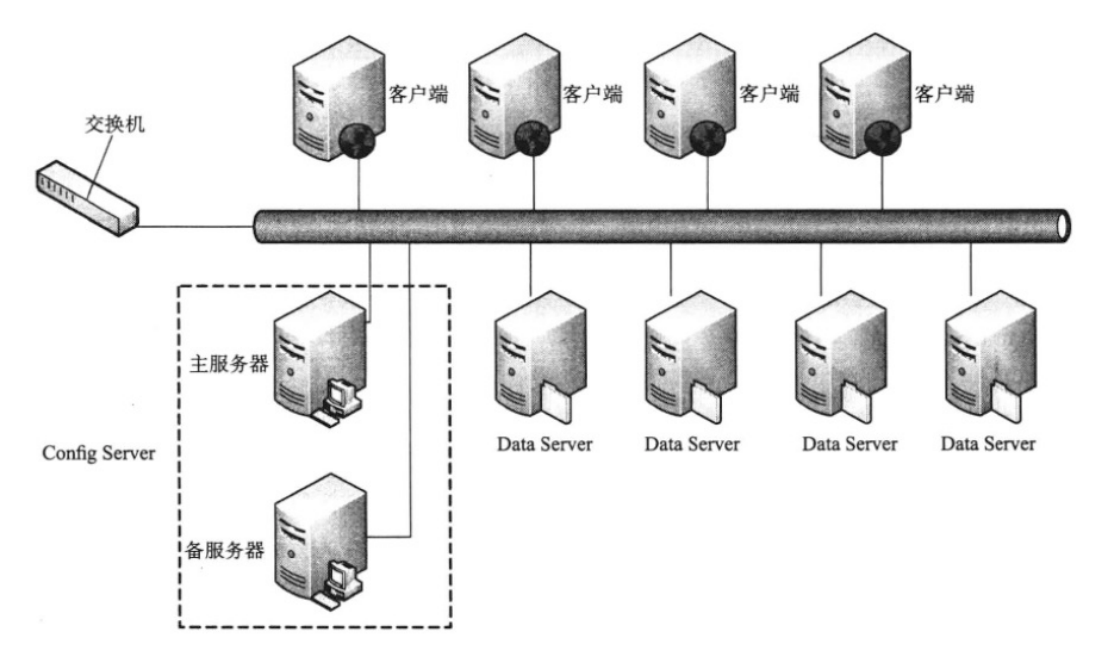
\includegraphics[width=\linewidth,height=.61\paperheight,keepaspectratio]{assets/source-2025/tair.png}
\column{.33\textwidth}
\begin{itemize}\item Config Server 维护配置与路由；\item 主/备配置节点形成独立故障边界；\item 多个 Data Server 承载数据分片；\item 客户端依据配置访问目标节点。\end{itemize}
\callout{观察}{“一个 key 的读写”背后可能跨越路由、分片和副本协议。}
\end{columns}
\end{frame}

% 14
\begin{frame}{案例四：OceanBase 的关系数据库架构}
\begin{columns}[T,onlytextwidth]
\column{.64\textwidth}
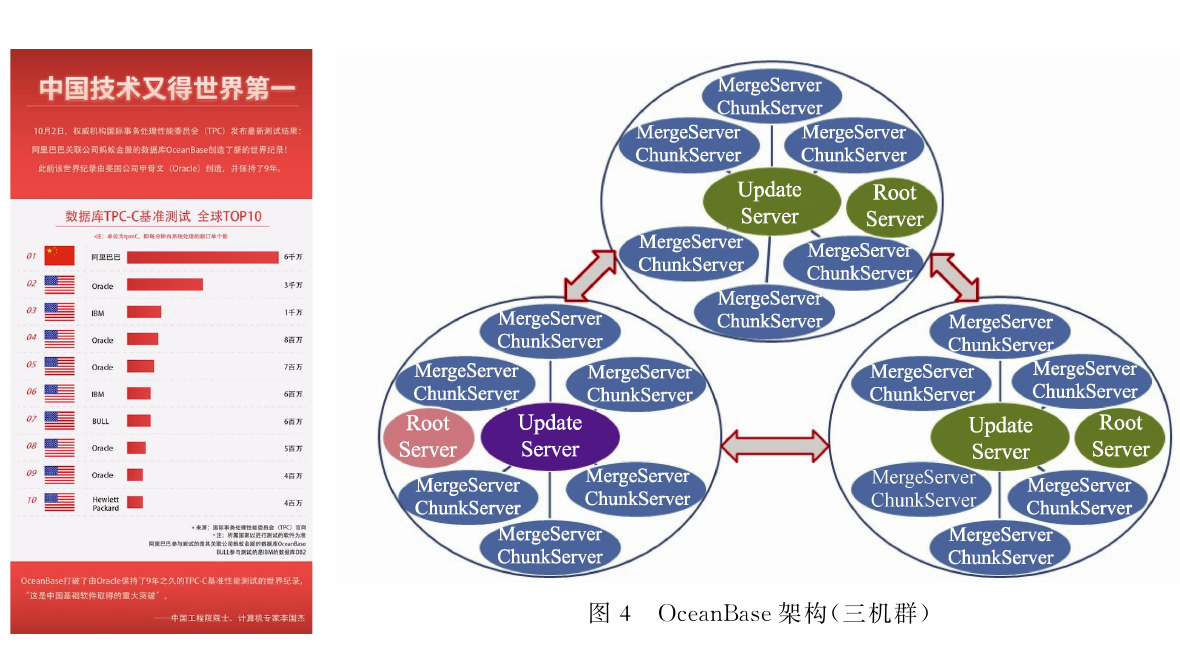
\includegraphics[width=\linewidth,height=.61\paperheight,keepaspectratio]{assets/source-2025/oceanbase.png}
\column{.31\textwidth}
\begin{itemize}
  \item 三机群之间协作；
  \item Root Server 管理元数据；
  \item Update Server 处理更新；
  \item Merge/Chunk Server 承担查询与数据组织。
\end{itemize}
\smallnote{原图引自阳振坤《OceanBase 关系数据库架构》。}
\end{columns}
\end{frame}

% 15
\begin{frame}{案例五：Elasticsearch 搜索集群}
\begin{columns}[T,onlytextwidth]
\column{.52\textwidth}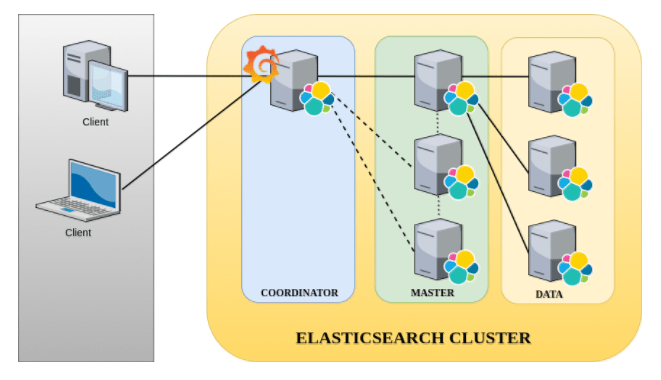
\includegraphics[width=\linewidth,height=.58\paperheight,keepaspectratio]{assets/elasticsearch.png}
\column{.42\textwidth}
\blocktitle{从图中读出系统语义}
\begin{enumerate}\item Client 只面对集群入口；\item Coordinator/Master 负责协调与元数据；\item Data 节点保存分片并执行查询；\item 复制与重新分片影响可用性和延迟。\end{enumerate}
\callout{互动}{如果一个 Data 节点变慢，应该“隐藏”还是“暴露”这个事实？}
\end{columns}
\end{frame}

\begin{frame}{案例六：边缘计算连接云、边缘与物联网}
\begin{columns}[T,onlytextwidth]
\column{.57\textwidth}
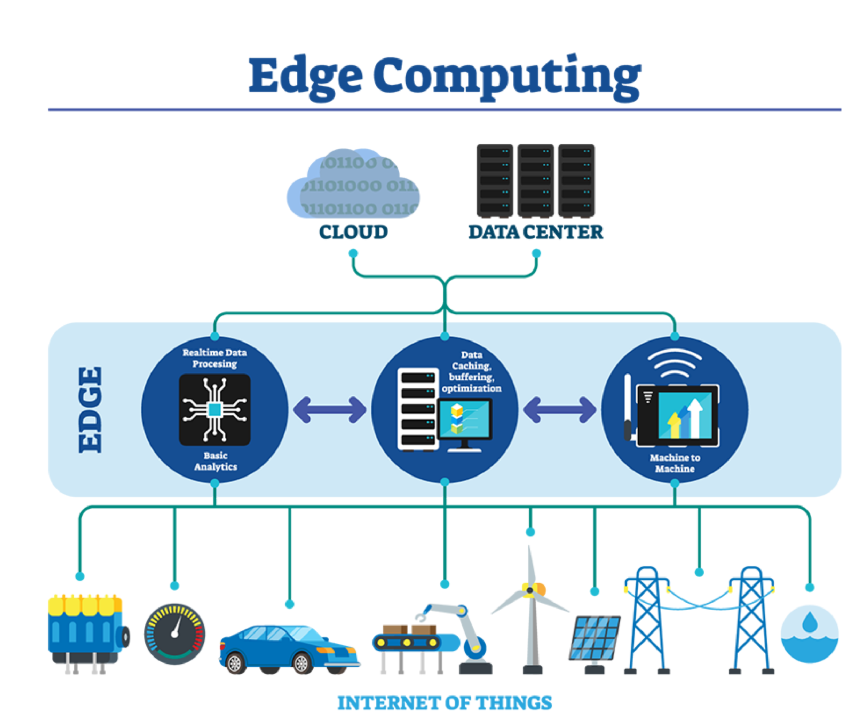
\includegraphics[width=\linewidth,height=.62\paperheight,keepaspectratio]{assets/source-2025/edge-computing.png}
\column{.38\textwidth}
\begin{itemize}
  \item 云/数据中心提供集中训练、全局数据与大规模资源；
  \item 边缘节点进行实时处理、缓存、优化和机器间协作；
  \item 终端包括车辆、工厂、电网、水务与可再生能源设施；
  \item 关键约束是时延、带宽、移动性、能耗与间歇连接。
\end{itemize}
\end{columns}
\end{frame}

% 16
\begin{frame}{案例七：大规模深度学习把“通信”变成主路径}
\begin{columns}[T,onlytextwidth]
\column{.58\textwidth}
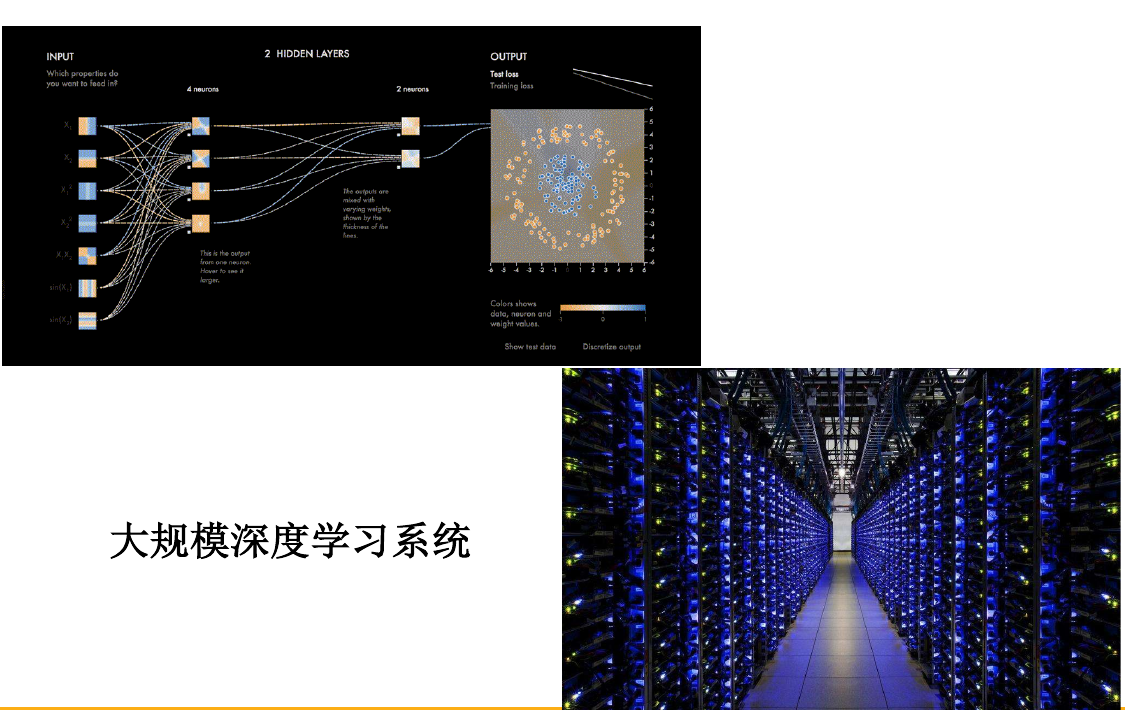
\includegraphics[width=\linewidth,height=.60\paperheight,keepaspectratio]{assets/source-2025/large-dl.png}
\column{.37\textwidth}
\begin{itemize}
  \item 单个模型训练由大量计算节点共同完成；
  \item 计算可并行，但同步点会放大尾延迟；
  \item 网络拓扑、显存和通信库共同决定有效吞吐；
  \item 故障恢复需要检查点、重调度与数据状态管理。
\end{itemize}
\end{columns}
\end{frame}

\begin{frame}{案例八：ChatGPT 与 Ray 的分布式运行时视角}
\begin{columns}[T,onlytextwidth]
\column{.60\textwidth}
\begin{center}
\begin{tikzpicture}[font=\small,>=Latex,scale=.82,transform shape]
  \node[draw=ADSBlue,fill=ADSLightBlue,rounded corners,minimum width=6.8cm,minimum height=.78cm] (app) {大模型应用：训练、微调、评测、在线服务};
  \node[draw=ADSOrange,fill=ADSOrange!12,rounded corners,minimum width=6.8cm,minimum height=1.15cm,below=7mm of app,align=center] (air)
    {Ray AI 工具层\\[-1mm]\scriptsize 数据处理｜训练｜调参｜服务｜强化学习};
  \node[draw=ADSGreen,fill=ADSGreen!10,rounded corners,minimum width=6.8cm,minimum height=1.15cm,below=7mm of air,align=center] (core)
    {Ray 核心运行时\\[-1mm]\scriptsize 任务（Task）｜有状态执行体（Actor）｜分布式对象（Object）};
  \node[draw=ADSGray,fill=ADSLightGray,rounded corners,minimum width=6.8cm,minimum height=.78cm,below=7mm of core] (cluster) {CPU / GPU 集群、网络与对象存储};
  \draw[\arrow,ADSGray] (app)--(air);\draw[\arrow,ADSGray] (air)--(core);\draw[\arrow,ADSGray] (core)--(cluster);
\end{tikzpicture}
\end{center}
\column{.35\textwidth}
\begin{itemize}
  \item Ray AIR：Data、Train、Tune、Serve、RLlib；
  \item Ray Core：Tasks、Actors、Objects；
  \item 目标是在 Python 抽象中组织可扩展 AI 工作负载；
  \item 运行时仍需解决调度、对象传输、故障与资源隔离。
\end{itemize}
\end{columns}
\end{frame}

% 17
\begin{frame}{Meta AI 基础设施：系统是软硬件共同设计}
\begin{columns}[T,onlytextwidth]
\column{.55\textwidth}
\begin{center}
\begin{tikzpicture}[font=\small,node distance=5mm,scale=.82,transform shape]
  \node[draw=ADSBlue,fill=ADSLightBlue,rounded corners,minimum width=6.1cm,minimum height=.75cm] (model) {模型与业务：Llama、推荐、生成式服务};
  \node[draw=ADSOrange,fill=ADSOrange!12,rounded corners,minimum width=6.1cm,minimum height=.75cm,below=of model] (soft) {系统软件：训练、推理、调度、可观测性};
  \node[draw=ADSGreen,fill=ADSGreen!10,rounded corners,minimum width=6.1cm,minimum height=.75cm,below=of soft] (store) {数据与存储：数据集、检查点、模型权重};
  \node[draw=ADSBlue,fill=ADSLightBlue,rounded corners,minimum width=6.1cm,minimum height=.75cm,below=of store] (net) {集群互联：RDMA / InfiniBand / 以太网};
  \node[draw=ADSGray,fill=ADSLightGray,rounded corners,minimum width=6.1cm,minimum height=.75cm,below=of net] (rack) {机架与节点：GPU、NVLink、CPU、SSD};
  \foreach \a/\b in {model/soft,soft/store,store/net,net/rack}{\draw[<->,ADSGray] (\a)--(\b);}
\end{tikzpicture}
\end{center}
\column{.39\textwidth}\begin{itemize}\item 机架内：GPU、互联、存储；\item 集群间：RDMA / InfiniBand 等网络；\item 软件层：训练、推理、调度和存储；\item 顶层：模型服务与业务流量。\end{itemize}\callout{读图方式}{不要只看“用了多少 GPU”，要看瓶颈位于计算、互联、存储还是调度。}\end{columns}
\end{frame}

% 18
\begin{frame}{DeepSeek 案例：H800 节点与多平面互联}
\begin{columns}[T,onlytextwidth]
\column{.51\textwidth}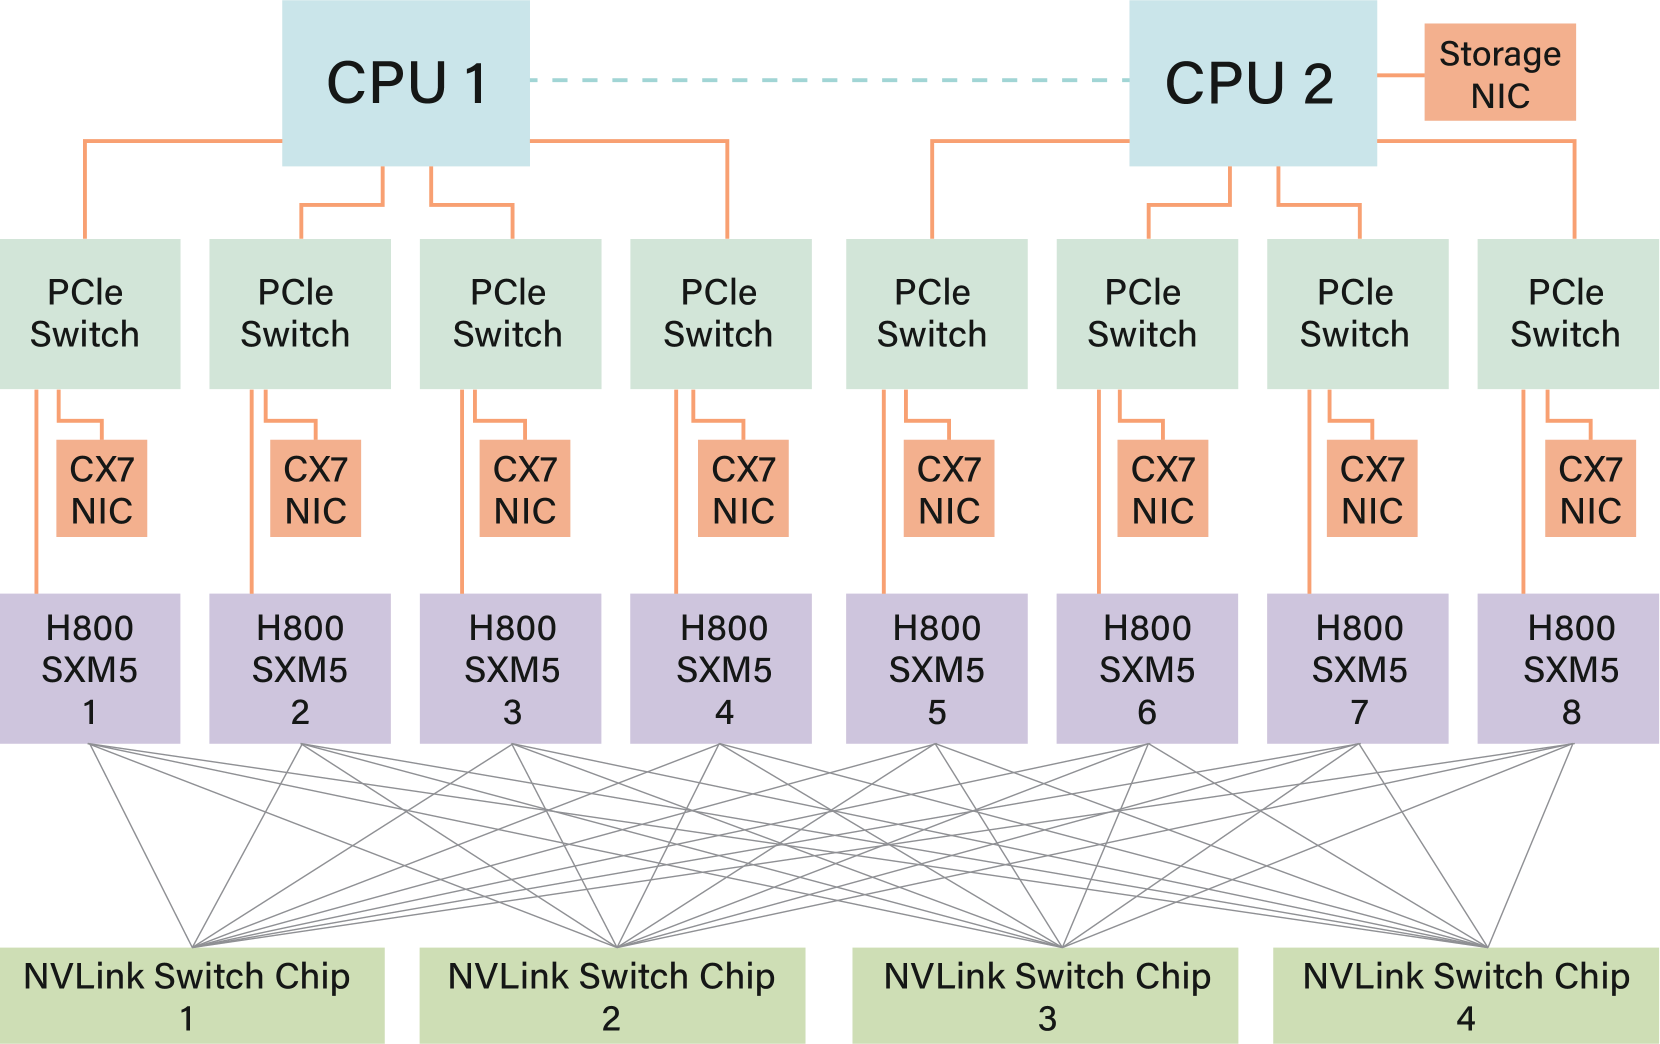
\includegraphics[width=\linewidth,height=.60\paperheight,keepaspectratio]{assets/h800-node.png}
\column{.44\textwidth}\begin{itemize}\item 节点内互联：GPU、NVLink、CPU/内存；\item 节点间连接：多平面网络与 RDMA；\item 训练效率取决于计算/通信重叠程度；\item 故障域要区分 GPU、节点、交换机和链路。\end{itemize}\end{columns}
\smallnote{H800 拓扑是大规模深度学习系统的典型案例；这里用“故障域—带宽—同步”解释。}
\end{frame}

% 19
\begin{frame}{NVLink：局部高速互联如何改变算法设计}
\begin{columns}[T,onlytextwidth]
\column{.50\textwidth}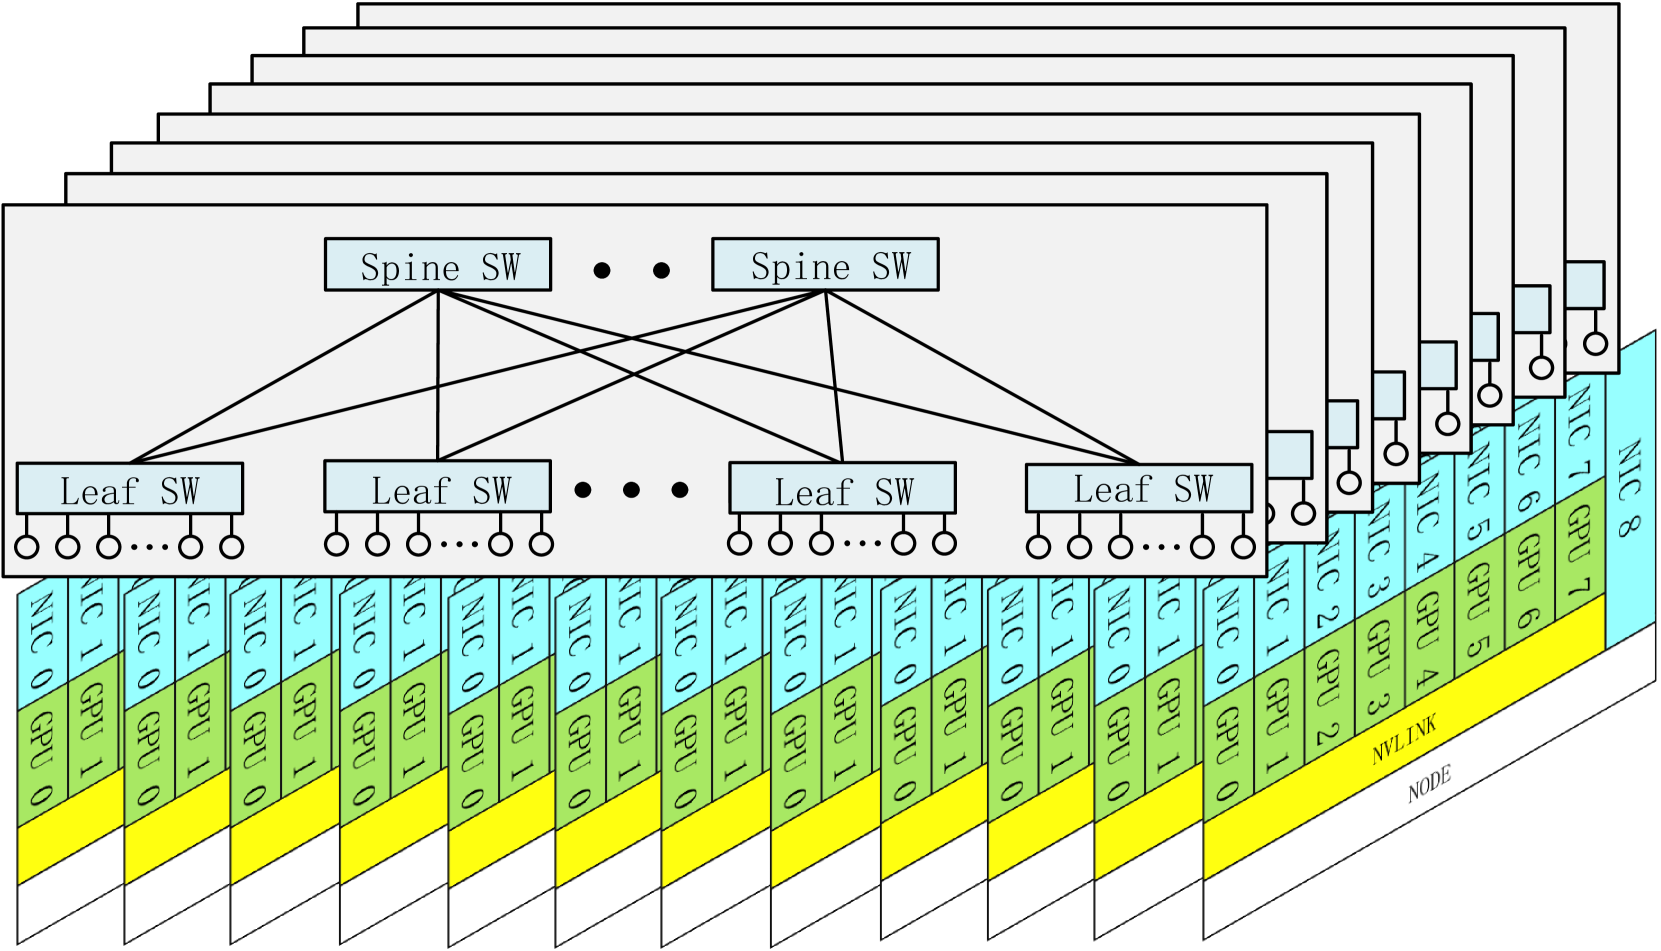
\includegraphics[width=\linewidth,height=.55\paperheight,keepaspectratio]{assets/nvlink.png}
\column{.45\textwidth}\begin{itemize}\item 近邻 GPU 的通信代价低于跨节点通信；\item 拓扑影响 AllReduce、张量并行和流水线并行；\item “统一 GPU 池”是抽象，实际是多级网络；\item 调度器需要感知拓扑，而不是只看空闲卡数。\end{itemize}\end{columns}
\end{frame}

\begin{frame}{NVLink 拓扑：PCIe 与 GPU 高速互联并存}
\begin{columns}[T,onlytextwidth]
\column{.58\textwidth}
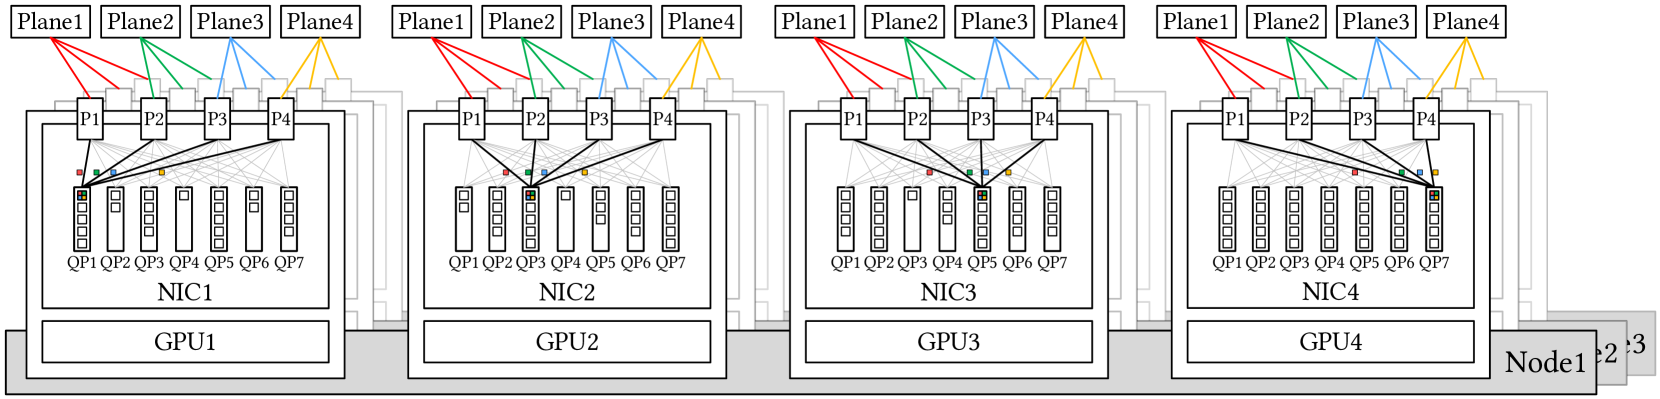
\includegraphics[width=\linewidth,height=.62\paperheight,keepaspectratio]{assets/nvlink-topology.png}
\column{.37\textwidth}
\begin{itemize}
  \item CPU 通过 PCIe Switch 连接 GPU；
  \item GPU 之间通过 NVLink 形成更高带宽路径；
  \item 不同 GPU 对之间的通信路径与代价并不相同；
  \item 拓扑感知放置与集合通信算法可避免跨越慢链路。
\end{itemize}
\end{columns}
\end{frame}

% 20
\begin{frame}{Kubernetes 推理：从请求到可扩展模型副本}
\begin{columns}[T,onlytextwidth]
\column{.55\textwidth}
\begin{center}
\begin{tikzpicture}[font=\scriptsize,>=Latex,node distance=6mm,scale=.82,transform shape]
  \nodebox[minimum width=3.0cm]{ADSBlue}{req}{客户端请求};
  \nodebox[below=of req,minimum width=3.0cm]{ADSOrange}{gateway}{推理网关：识别模型};
  \nodebox[below=of gateway,minimum width=3.0cm]{ADSBlue}{sched}{调度器：读取负载与缓存};
  \node[draw=ADSGreen,fill=ADSGreen!10,rounded corners,minimum width=5.0cm,minimum height=1.05cm,below=of sched,align=center] (pool)
    {推理实例池\\预填充副本｜解码副本｜前缀缓存};
  \nodebox[left=7mm of pool,minimum width=2.0cm]{ADSOrange}{auto}{弹性伸缩};
  \draw[\arrow,ADSGray] (req)--(gateway);\draw[\arrow,ADSGray] (gateway)--(sched);
  \draw[\arrow,ADSGray] (sched)--(pool);
  \draw[\arrow,ADSOrange] (auto)--(pool);
\end{tikzpicture}
\end{center}
\column{.40\textwidth}\begin{itemize}\item Client $\rightarrow$ Inference Gateway；\item 根据模型名选择 InferencePool；\item Scheduler 结合负载与 KV Cache 选择副本；\item Autoscaler 根据容量边界调整副本数。\end{itemize}\callout{关键取舍}{路由、调度、缓存和弹性必须共享同一套可观测状态。}\end{columns}
\end{frame}

% 21
\begin{frame}{Kubernetes 推理架构：组件之间如何协同}
\begin{center}
\begin{tikzpicture}[node distance=7mm and 8mm,scale=.80,transform shape]
\nodebox{ADSBlue}{client}{客户端};\nodebox[right=of client]{ADSOrange}{gw}{推理网关};
\node[draw=ADSBlue,fill=ADSLightBlue,rounded corners,minimum width=3.0cm,minimum height=.75cm,right=of gw] (route) {请求体路由};
\node[draw=ADSGreen,fill=ADSGreen!10,rounded corners,minimum width=4.1cm,minimum height=1.1cm,right=of route,align=center] (pool) {推理实例池\\方案 A：预填充\quad 方案 B：解码};
\node[draw=ADSBlue,fill=ADSLightBlue,rounded corners,minimum width=3.0cm,minimum height=.75cm,below=10mm of route] (sched) {推理调度器};
\node[draw=ADSOrange,fill=ADSOrange!12,rounded corners,minimum width=3.0cm,minimum height=.75cm,below=10mm of sched] (scale) {实例弹性伸缩器};
\node[draw=ADSGray,fill=ADSLightGray,rounded corners,minimum width=4.1cm,minimum height=.62cm,below=of pool] (cache) {共享 / 独立的前缀缓存};
\draw[ADSBlue,\arrow] (client)--(gw);\draw[ADSOrange,\arrow] (gw)--(route);\draw[ADSBlue,\arrow] (route)--(pool);\draw[ADSBlue,\arrow] (sched.east)--(pool.west);\draw[ADSOrange,\arrow,dashed,bend left=24] (scale.east) to (pool.south west);\draw[ADSGray,\arrow,bend left=10] (pool)--(cache);\draw[ADSGray,\arrow,bend left=10] (cache)--(pool);
\end{tikzpicture}
\end{center}
\smallnote{调度器根据负载和 KV 缓存状态选择实例；伸缩器改变副本数；前缀缓存减少预填充阶段的重复计算。}
\end{frame}

% 22
\begin{frame}{大模型训练与推理：复杂的软件栈}
\begin{columns}[T,onlytextwidth]
\column{.52\textwidth}
\begin{center}
\begin{tikzpicture}[font=\small,node distance=4mm,scale=.83,transform shape]
  \node[draw=ADSBlue,fill=ADSLightBlue,rounded corners,minimum width=5.7cm,minimum height=.72cm] (m) {模型与业务：Transformer、RAG、智能体};
  \node[draw=ADSOrange,fill=ADSOrange!12,rounded corners,minimum width=5.7cm,minimum height=.72cm,below=of m] (f) {框架与运行时：训练、推理、批处理};
  \node[draw=ADSGreen,fill=ADSGreen!10,rounded corners,minimum width=5.7cm,minimum height=.72cm,below=of f] (c) {通信：集合通信、RDMA、RPC};
  \node[draw=ADSBlue,fill=ADSLightBlue,rounded corners,minimum width=5.7cm,minimum height=.72cm,below=of c] (o) {编排：Kubernetes、队列、监控};
  \node[draw=ADSGray,fill=ADSLightGray,rounded corners,minimum width=5.7cm,minimum height=.72cm,below=of o] (r) {资源：GPU、网络、存储};
  \foreach \a/\b in {m/f,f/c,c/o,o/r}{\draw[<->,ADSGray] (\a)--(\b);}
\end{tikzpicture}
\end{center}
\column{.43\textwidth}\begin{enumerate}\item 模型层：Transformer、权重、KV Cache；\item 框架层：训练/推理运行时；\item 通信层：集合通信、RDMA、RPC；\item 编排层：Kubernetes、作业队列、监控；\item 资源层：GPU、网络、存储。\end{enumerate}\end{columns}
\end{frame}

% 23
\begin{frame}{微服务系统：网络调用就是程序控制流的一部分}
\begin{columns}[T,onlytextwidth]
\column{.61\textwidth}
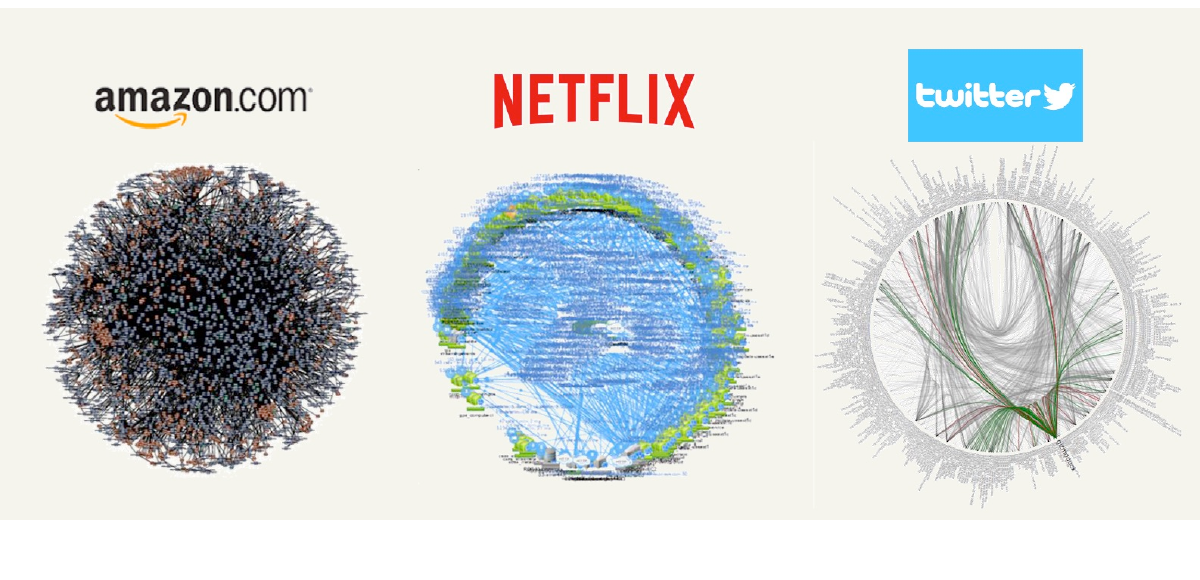
\includegraphics[width=\linewidth,height=.58\paperheight,keepaspectratio]{assets/source-2025/microservices.png}
\column{.34\textwidth}
\begin{itemize}
  \item 服务数量和依赖边快速增长；
  \item 一次请求包含多个潜在故障点；
  \item 可观测性必须跨服务传播 trace/span；
  \item 重试可能把局部故障放大成级联故障。
\end{itemize}
\end{columns}
\end{frame}

\begin{frame}{分布式应用、操作系统、中间件与协议栈}
\begin{columns}[T,onlytextwidth]
\column{.59\textwidth}
\begin{center}
\begin{tikzpicture}[font=\small,scale=.72,transform shape]
  \node[draw=ADSBlue,fill=ADSLightBlue,rounded corners,minimum width=6.7cm,minimum height=.75cm] (app) {分布式应用};
  \node[draw=ADSOrange,fill=ADSOrange!12,rounded corners,minimum width=5.9cm,minimum height=.85cm,below=5mm of app] (mid) {中间件与分布式运行时};
  \node[draw=ADSGreen,fill=ADSGreen!10,rounded corners,minimum width=2.8cm,minimum height=2.5cm,below left=5mm and 1mm of mid,align=center] (os) {操作系统\\进程 / 内存 / 文件};
  \node[draw=ADSGray,fill=ADSLightGray,rounded corners,minimum width=2.8cm,minimum height=2.5cm,below right=5mm and 1mm of mid,align=center] (net) {网络协议栈\\应用层\\传输层\\网络层 / 链路层};
  \draw[\arrow,ADSGray] (app)--(mid);\draw[\arrow,ADSGray] (mid)--(os);\draw[\arrow,ADSGray] (mid)--(net);
\end{tikzpicture}
\end{center}
\column{.36\textwidth}
\begin{itemize}
  \item 分布式应用调用中间件库；
  \item 中间件与操作系统共同使用网络协议栈；
  \item 分布式协议可能跨越应用、中间件和传输层；
  \item 抽象边界决定故障处理和性能优化的位置。
\end{itemize}
\end{columns}
\end{frame}

\begin{frame}{为什么构建分布式系统？}
\begin{columns}[T,onlytextwidth]
\column{.48\textwidth}
\begin{itemize}
  \item 计算任务本身天然分布；
  \item 共享资源与访问远程资源；
  \item 提高性能/成本比；
  \item 模块化与增量扩展。
\end{itemize}
\column{.48\textwidth}
\begin{itemize}
  \item 可靠性：可用性、完整性、容错；
  \item 可扩展性：规模、地域与管理域；
  \item 在独立故障边界之间建立统一服务；
  \item 让资源在网络上可访问和可组合。
\end{itemize}
\end{columns}
\vfill
\callout{代价}{这些收益都以通信延迟、并发控制、局部故障和运维复杂性为代价。}
\end{frame}

% 24
\begin{frame}{超级计算机与分布式系统：同一张谱系中的不同位置}
\begin{columns}[T,onlytextwidth]
\column{.48\textwidth}
\blocktitle{Tianhe I / II 等系统}
\begin{itemize}\item 大规模节点、专用互联、集中式作业调度；\item 追求可预测的吞吐和浮点性能；\item 通信拓扑与并行算法紧密耦合。\end{itemize}
\column{.48\textwidth}
\blocktitle{云与互联网系统}
\begin{itemize}\item 负载动态、服务多租户、故障常态化；\item 追求弹性、可用性、成本与用户延迟；\item 抽象层更多，系统边界更模糊。\end{itemize}
\end{columns}
\vfill\callout{共同问题}{并行性、通信、调度、故障与性能测量；不同的是假设和优化目标。}
\end{frame}

% 25
\begin{frame}{为什么今天仍然需要分布式系统基础}
\begin{center}
\begin{tikzpicture}[node distance=8mm]
\node[draw=ADSBlue,fill=ADSLightBlue,rounded corners,minimum width=2.6cm,minimum height=.8cm] (scale) {规模增长};
\node[draw=ADSOrange,fill=ADSOrange!12,rounded corners,minimum width=2.6cm,minimum height=.8cm,right=of scale] (lat) {延迟约束};
\node[draw=ADSGreen,fill=ADSGreen!10,rounded corners,minimum width=2.6cm,minimum height=.8cm,right=of lat] (fail) {故障常态};
\node[draw=ADSGray,fill=ADSLightGray,rounded corners,minimum width=2.6cm,minimum height=.8cm,right=of fail] (trust) {数据与权限};
\draw[ADSBlue,\arrow] (scale)--(lat);\draw[ADSOrange,\arrow] (lat)--(fail);\draw[ADSGreen,\arrow] (fail)--(trust);
\end{tikzpicture}
\end{center}
\vfill\begin{itemize}\item 云计算、云原生、无服务器、在网计算、算力网络、智算中心、区块链和大模型，都把分布式假设推到前台。\item 课程不追逐产品名词，而是追问它们共享的系统问题。\end{itemize}
\end{frame}

\sectionframe{并行系统与互联结构}{共享内存、消息传递和网络拓扑共同决定计算的粒度与代价。}

\begin{frame}{并行系统的三种典型组织方式}
\small
\begin{itemize}
  \item \key{多处理器系统}：处理器直接访问共享内存（典型 UMA）；互联可采用总线或多级交换网络，如 Omega、Butterfly、Clos、Shuffle-exchange。
  \item \key{多计算机并行系统}：节点不直接访问同一物理内存；互联可采用总线、环、网格、环面和超立方体。这里区分“非均匀共享内存”与“分布式内存”。
  \item \key{阵列处理器}：紧耦合、共同时钟、协同执行，常见于专用 DSP/向量工作负载。
\end{itemize}
\vfill
\callout{设计变量}{互联生成函数、路由函数、网络直径、割带宽以及是否允许局部缓存。}
\end{frame}

\begin{frame}{UMA 与 NUMA：访问语义相同，访问代价不同}
\begin{columns}[T,onlytextwidth]
\column{.58\textwidth}
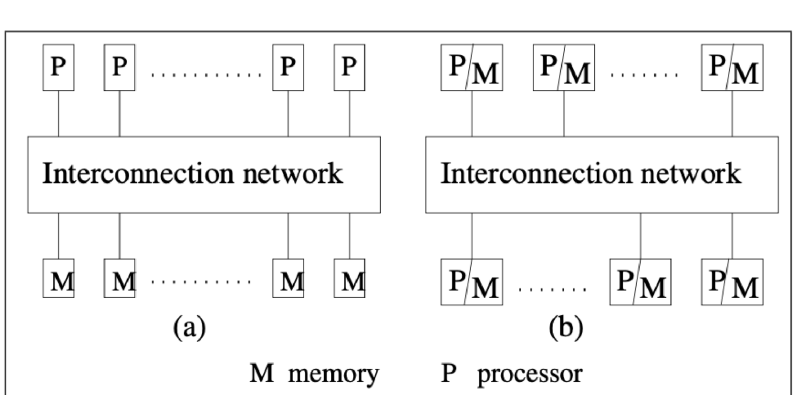
\includegraphics[width=\linewidth,height=.54\paperheight,keepaspectratio]{assets/source-2025/uma-numa.png}
\column{.37\textwidth}
\begin{itemize}
  \item UMA：处理器到各内存模块的访问代价近似一致；
  \item NUMA：处理器拥有邻近内存，远端访问更昂贵；
  \item 两者都可能缓存共享数据；
  \item 一致性协议必须处理副本和并发写入。
\end{itemize}
\end{columns}
\smallnote{M 表示 memory，P 表示 processor。}
\end{frame}

\begin{frame}{Omega 与 Butterfly：多级互联网络}
\begin{center}
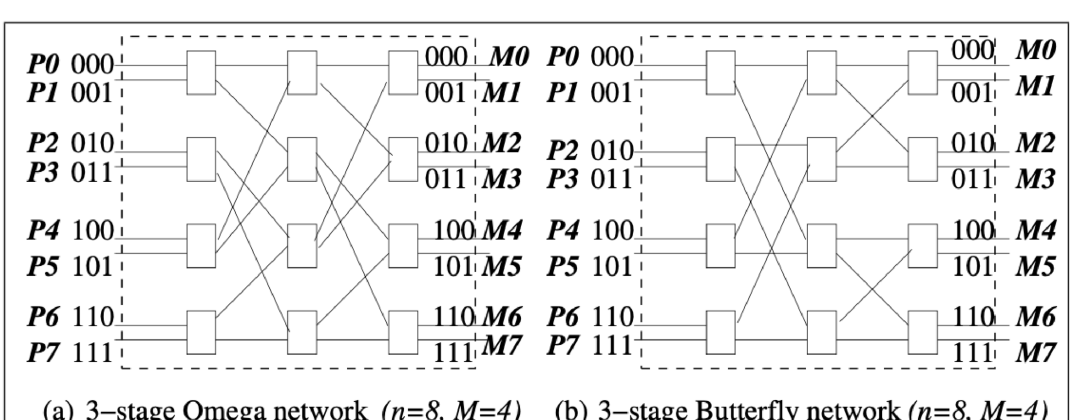
\includegraphics[width=.88\linewidth,height=.54\paperheight,keepaspectratio]{assets/source-2025/omega-butterfly.png}
\end{center}
\vfill
\begin{columns}[T,onlytextwidth]
\column{.48\textwidth}\callout{Omega}{级间采用 perfect shuffle，目的地址位逐级决定交换方向。}
\column{.48\textwidth}\callout{Butterfly}{同样使用多级 $2\times2$ 交换单元，但级间连线模式不同。}
\end{columns}
\end{frame}

\begin{frame}{Omega Network：生成函数与逐位路由}
\begin{columns}[T,onlytextwidth]
\column{.48\textwidth}
\blocktitle{结构}
\begin{itemize}
  \item $n$ 个处理器、$n$ 个内存模块；
  \item $\log_2 n$ 级；
  \item 每级包含 $n/2$ 个 $2\times2$ 交换单元。
\end{itemize}
\column{.48\textwidth}
\blocktitle{级间连接函数}
\[
j=\begin{cases}
2i,&0\le i\le n/2-1,\\
2i+1-n,&n/2\le i\le n-1.
\end{cases}
\]
\end{columns}
\vfill
\callout{路由规则}{在第 $s$ 级查看目的地址 $j$ 的第 $s+1$ 个最高有效位：0 走上支路，1 走下支路。}
\end{frame}

\begin{frame}{Mesh、Torus 与 Hypercube 拓扑}
\begin{columns}[T,onlytextwidth]
\column{.62\textwidth}
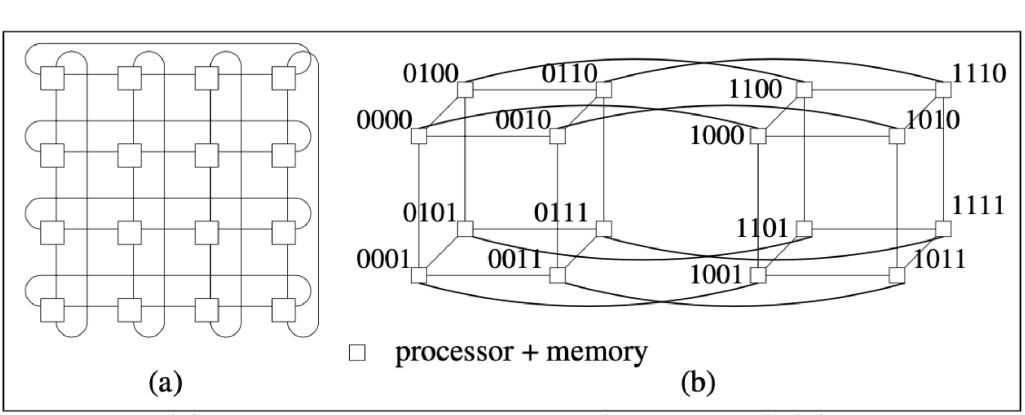
\includegraphics[width=\linewidth,height=.54\paperheight,keepaspectratio]{assets/source-2025/mesh-hypercube.png}
\column{.33\textwidth}
\begin{itemize}
  \item 2-D Mesh：布局规则、局部连接；
  \item Torus：在网格边界增加回绕链路；
  \item $d$ 维 Hypercube：$2^d$ 个节点；
  \item 节点以二进制编号，汉明距离为 1 的节点相连。
\end{itemize}
\end{columns}
\smallnote{拓扑影响直径、节点度、割带宽、布线复杂度与路由容错。}
\end{frame}

% 26
\begin{frame}{Flynn 分类：为什么 MIMD 是分布式系统的常见视角}
\begin{center}\scriptsize
\begin{tabular}{c|c|c|c}
\toprule 模式 & 指令流 & 数据流 & 典型场景 \\
\midrule
SISD & 单 & 单 & 传统单处理器 \\
SIMD & 单 & 多 & 向量处理、科学计算 \\
MISD & 多 & 单 & 少见的专用流水 \\
MIMD & 多 & 多 & 多数并行与分布式系统 \\
\bottomrule
\end{tabular}
\end{center}
\vfill\callout{注意}{MIMD 只是硬件/执行视角；分布式系统还要定义通信、故障和对外语义。}
\end{frame}

% 27
\begin{frame}{术语：耦合、并行性、并发性、粒度}
\begin{columns}[T,onlytextwidth]
\column{.48\textwidth}\begin{itemize}\item \term{耦合}{Coupling}：模块之间的依赖与绑定；\item \term{并行性}{Parallelism}：$T(1)/T(n)$，取决于程序与系统；\item \term{并发性}{Concurrency}：生产性 CPU 时间与同步等待的关系。\end{itemize}
\column{.48\textwidth}\begin{itemize}\item \term{粒度}{Granularity}：计算量与通信量之比；\item 粗粒度适合松耦合系统；\item 细粒度需要低延迟、高带宽互联。\end{itemize}\end{columns}
\vfill\begin{tikzpicture}\draw[ADSBlue,very thick] (0,0)--(5,0) node[right,font=\scriptsize]{计算/通信比};\draw[ADSOrange,fill=ADSOrange] (1.5,0) circle (2pt) node[above,font=\scriptsize]{细粒度};\draw[ADSGreen,fill=ADSGreen] (4.2,0) circle (2pt) node[above,font=\scriptsize]{粗粒度};\end{tikzpicture}
\end{frame}

% 28
\begin{frame}{系统比较：集中、并行、分布式与 P2P}
\begin{center}\scriptsize
\begin{tabular}{>{\bfseries}p{2.3cm}p{3.0cm}p{3.0cm}p{3.0cm}}
\toprule 维度 & 集中式 & 并行式 & 分布式 / P2P \\
\midrule
控制 & 单点集中 & 作业/硬件协同 & 多节点自治 \\
通信 & 本地调用 & 高速专用互联 & 网络消息与不确定延迟 \\
故障 & 较易定位 & 通常受控 & 故障与慢节点难区分 \\
目标 & 简单性 & 性能 & 规模、可用性、地域与开放性 \\
\bottomrule
\end{tabular}
\end{center}
\vfill\smallnote{MPI、MapReduce、OpenMP/TBB 等工具位于不同的抽象层，不能用一个“分布式/非分布式”标签简单归类。}
\end{frame}

% 29
\begin{frame}{消息传递与共享内存：两种基本抽象}
\begin{columns}[T,onlytextwidth]
\column{.47\textwidth}
\blocktitle{Message Passing（MP）}
\begin{tikzpicture}[node distance=8mm]\nodebox{ADSBlue}{p1}{进程 P1};\nodebox[right=of p1]{ADSBlue}{p2}{进程 P2};\draw[ADSOrange,\arrow,bend left=12] (p1) to node[above,font=\scriptsize]{send} (p2);\draw[ADSBlue,\arrow,bend left=12] (p2) to node[below,font=\scriptsize]{reply} (p1);\end{tikzpicture}
\begin{itemize}\item 显式通信；\item 消息顺序、丢失和重试成为协议。\end{itemize}
\column{.47\textwidth}
\blocktitle{Shared Memory（SM）}
\begin{tikzpicture}[node distance=8mm]\nodebox{ADSBlue}{q1}{进程 P1};\nodebox[right=of q1]{ADSBlue}{q2}{进程 P2};\node[draw=ADSOrange,fill=ADSOrange!12,rounded corners,minimum width=2.2cm,minimum height=.7cm,below=of q1,xshift=1.5cm] (mem) {共享对象};\draw[ADSOrange,\arrow] (q1)--(mem);\draw[ADSOrange,\arrow] (q2)--(mem);\end{tikzpicture}
\begin{itemize}\item 隐式通信；\item 一致性、原子性和同步成为协议。\end{itemize}
\end{columns}
\end{frame}

% 30
\begin{frame}{系统仿真：MP 与 SM 可以互相模拟}
\begin{center}
\begin{tikzpicture}[node distance=38mm]
\node[draw=ADSBlue,fill=ADSLightBlue,rounded corners,minimum width=3.5cm,minimum height=.8cm] (mp) {Message Passing};
\node[draw=ADSOrange,fill=ADSOrange!12,rounded corners,minimum width=3.5cm,minimum height=.8cm,right=of mp] (sm) {Shared Memory};
\draw[ADSBlue,\arrow,bend left=24] (mp) to node[above,font=\tiny,fill=white,inner sep=1pt]{共享对象由所有者进程管理} (sm);
\draw[ADSOrange,\arrow,bend left=24] (sm) to node[below,font=\tiny,fill=white,inner sep=1pt]{mailbox + send/receive} (mp);
\end{tikzpicture}
\end{center}
\vfill\begin{itemize}\item 在 MP 上模拟 SM：为每个共享对象设一个所有者进程。\item 在 SM 上模拟 MP：为每对进程划分 mailbox。\item 仿真不会免费带来性能；它只改变“可证明/可编程”的边界。\end{itemize}
\end{frame}

% 31
\begin{frame}{原语分类一：同步/异步描述 Send 的完成条件}
\begin{columns}[T,onlytextwidth]
\column{.47\textwidth}
\blocktitle{同步 Send（Synchronous）}
\begin{itemize}
  \item 发送方与接收方完成握手；
  \item Send 在匹配的 Receive 完成时才完成；
  \item Receive 在数据复制进接收缓冲区后完成。
\end{itemize}
\column{.47\textwidth}
\blocktitle{异步 Send（Asynchronous）}
\begin{itemize}
  \item 数据复制出发送方指定的用户缓冲区后，Send 即可完成；
  \item 完成不代表接收方已经收到；
  \item 发送缓冲区可安全复用。
\end{itemize}
\end{columns}
\vfill\callout{边界}{教材在此只把 Send 分为同步/异步；Receive 再按阻塞/非阻塞分类。}
\end{frame}

% 32
\begin{frame}{原语分类二：阻塞/非阻塞}
\begin{columns}[T,onlytextwidth]
\column{.47\textwidth}
\blocktitle{阻塞（Blocking）}
\begin{itemize}
  \item 调用进程在原语处理完成后才取回控制权；
  \item 对 Send 而言，完成条件仍取决于它是同步还是异步；
  \item 对 Receive 而言，数据进入用户缓冲区后返回。
\end{itemize}
\column{.47\textwidth}
\blocktitle{非阻塞（Nonblocking）}
\begin{itemize}
  \item 调用后立即返回句柄；
  \item Send 返回时，数据甚至可能尚未复制出用户缓冲区；
  \item Receive 返回时，消息甚至可能尚未到达。
\end{itemize}
\end{columns}
\vfill\callout{后续动作}{程序通过 Test/Wait 检查完成；Wait 本身是阻塞调用。}
\end{frame}

% 33
\begin{frame}{非阻塞发送：句柄把“完成”变成可观察状态}
\begin{columns}[T,onlytextwidth]
\column{.56\textwidth}
\begin{block}{伪代码}
\ttfamily\small
Send(X, destination, handle$_k$)\\
\dots\\
Wait(handle$_1$, handle$_2$, \dots, handle$_k$)\\
\end{block}
\column{.38\textwidth}\begin{itemize}\item 立即返回不代表网络已完成；\item 句柄用于查询状态；\item Wait 仍可能阻塞，但阻塞点由程序显式控制。\end{itemize}\end{columns}
\vfill\smallnote{设计提醒：异常路径必须定义句柄失效、超时、重复发送与资源回收。}
\end{frame}

% 34
\begin{frame}{四种 Send 原语：完成条件与进程阻塞}
\begin{center}
\begin{tikzpicture}[x=.92cm,y=.82cm]
\draw[->,ADSGray] (0,.65)--(10.4,.65) node[right,font=\scriptsize]{时间};
\foreach \y/\name in {0/{(a) 阻塞同步 Send},-1.35/{(b) 非阻塞同步 Send},-2.70/{(c) 阻塞异步 Send},-4.05/{(d) 非阻塞异步 Send}}{
  \draw[ADSGray!55] (0,\y)--(10,\y);
  \node[anchor=east,font=\scriptsize] at (-.15,\y) {\name};
}
\node[font=\scriptsize,ADSBlue] at (1,0.28) {$S$};
\draw[ADSOrange,line width=3pt] (1,0)--(7,0);
\node[font=\scriptsize,ADSBlue] at (7,0.28) {$S_C$};
\node[font=\tiny,anchor=south] at (4,0) {等待匹配 Receive 完成};

\node[font=\scriptsize,ADSBlue] at (1,-1.07) {$S$};
\draw[ADSBlue,dashed,line width=1pt] (1,-1.35)--(7,-1.35);
\node[font=\scriptsize,ADSOrange] at (5,-1.07) {$W$};
\draw[ADSOrange,line width=3pt] (5,-1.35)--(7,-1.35);
\node[font=\scriptsize,ADSBlue,anchor=west] at (7,-1.07) {$P,S_C$};

\node[font=\scriptsize,ADSBlue] at (1,-2.42) {$S$};
\draw[ADSGreen,line width=3pt] (1,-2.70)--(3.2,-2.70);
\draw[ADSOrange,line width=1.4pt] (1,-2.53)--(3.2,-2.53);
\node[font=\scriptsize,ADSBlue] at (3.2,-2.42) {$S_C$};
\node[font=\tiny,anchor=south] at (2.1,-2.70) {复制出用户缓冲区};

\node[font=\scriptsize,ADSBlue] at (1,-3.77) {$S$};
\draw[ADSGreen,line width=3pt] (1,-4.05)--(3.2,-4.05);
\node[font=\scriptsize,ADSOrange] at (2.4,-3.77) {$W$};
\draw[ADSOrange,line width=3pt] (2.4,-4.05)--(3.2,-4.05);
\node[font=\scriptsize,ADSBlue,anchor=west] at (3.2,-3.77) {$P,S_C$};
\end{tikzpicture}
\end{center}
\smallnote{橙色粗线：调用进程被阻塞；绿色粗线：数据复制出发送方用户缓冲区；虚线：非阻塞操作在后台尚未完成。}
\end{frame}

\begin{frame}{四种 Send 原语与 MPI 发送模式不要混淆}
\small
\begin{columns}[T,onlytextwidth]
\column{.48\textwidth}
\blocktitle{本讲的二维分类}
\begin{itemize}
  \item 同步/异步：描述 Send 何时算完成；
  \item 阻塞/非阻塞：描述调用是否立即把控制权还给程序；
  \item 四种组合只刻画“调用方可观察到的完成事件”；
  \item 具体实现还要说明缓冲区、匹配、取消和错误处理。
\end{itemize}
\column{.48\textwidth}
\blocktitle{MPI 中的另一组术语}
\begin{itemize}
  \item standard、buffered、synchronous、ready 是发送模式；
  \item 每种模式还可以有 blocking/nonblocking 变体；
  \item 因此“同步 Send”不等于“MPI\_Ssend”，更不能把四条时间线直接当成 MPI 全部语义；
  \item 读协议时必须先写清完成条件。
\end{itemize}
\end{columns}
\vfill
\callout{课堂判别}{看到一个 Send，先问“用户缓冲区何时可复用？接收方何时必须参与？调用何时返回？”再给它命名。}
\end{frame}

\begin{frame}{两种 Receive 原语：消息到达与控制返回}
\begin{center}
\begin{tikzpicture}[x=1.05cm,y=1cm]
\draw[->,ADSGray] (0,.65)--(9.7,.65) node[right,font=\scriptsize]{时间};
\draw[ADSGray!55] (0,0)--(9.3,0);
\draw[ADSGray!55] (0,-2)--(9.3,-2);
\node[anchor=east,font=\scriptsize] at (-.15,0) {阻塞 Receive};
\node[anchor=east,font=\scriptsize] at (-.15,-2) {非阻塞 Receive};

\node[font=\scriptsize,ADSBlue] at (1,0.3) {$R$};
\draw[ADSOrange,line width=3pt] (1,0)--(6,0);
\draw[ADSGreen,line width=3pt] (5,0)--(6,0);
\node[font=\scriptsize,ADSGray] at (5,.3) {消息到达};
\node[font=\scriptsize,ADSBlue] at (6,.3) {$R_C$};

\node[font=\scriptsize,ADSBlue] at (1,-1.7) {$R$};
\draw[ADSBlue,dashed,line width=1pt] (1,-2)--(6,-2);
\node[font=\scriptsize,ADSOrange] at (4.2,-1.7) {$W$};
\draw[ADSOrange,line width=3pt] (4.2,-2)--(6,-2);
\draw[ADSGreen,line width=3pt] (5,-2)--(6,-2);
\node[font=\scriptsize,ADSGray] at (5,-1.7) {消息到达};
\node[font=\scriptsize,ADSBlue,anchor=west] at (6,-1.7) {$P,R_C$};
\end{tikzpicture}
\end{center}
\begin{itemize}
  \item 阻塞 Receive 从 $R$ 一直等待到数据复制进用户缓冲区并产生 $R_C$；
  \item 非阻塞 Receive 立即返回，随后用 Wait/Test 获得完成事件 $P$；若操作已完成，Wait 可立即返回。
\end{itemize}
\end{frame}

% 35
\begin{frame}{异步执行：事件之间只有偏序关系}
\begin{center}\begin{tikzpicture}[x=1cm,y=0.65cm]
\foreach \y/\p in {0/P0,1/P1,2/P2,3/P3}{\draw[ADSGray] (0,-\y)--(10,-\y) node[left,font=\scriptsize]{\p};}
\foreach \x/\y/\l in {1/0/m1,3/1/m2,2/2/m3,5/2/m4,7/3/m5,8/1/m6,9/0/m7}{\fill[ADSBlue] (\x,-\y) circle (2pt) node[above,font=\tiny]{\l};}
\draw[ADSOrange,->] (1,-0.03)--(3,-0.97);\draw[ADSOrange,->] (2,-1.97)--(5,-2.03);\draw[ADSOrange,->] (5,-2.03)--(7,-2.97);\draw[ADSOrange,->] (7,-2.97)--(8,-1.03);\draw[ADSOrange,->] (8,-1.03)--(9,-0.03);
\end{tikzpicture}\end{center}
\vfill\begin{itemize}\item 每条进程线上的事件有先后；\item 不同进程事件之间通常只有因果约束；\item 全序需要额外协议，会引入通信和等待。\end{itemize}
\end{frame}

\begin{frame}{异步执行：三类事件共同形成 happened-before}
\begin{columns}[T,onlytextwidth]
\column{.30\textwidth}\callout{内部事件}{只改变一个进程的局部状态。}
\column{.30\textwidth}\callout{发送事件}{产生消息，并先于对应接收事件。}
\column{.30\textwidth}\callout{接收事件}{消费消息，改变接收进程状态。}
\end{columns}
\vfill
\begin{itemize}
  \item 同一进程中的程序顺序给出局部先后关系；
  \item 每条消息给出 $send(m) \rightarrow receive(m)$；
  \item 传递闭包形成偏序；两个互不可达的事件可以并发；
  \item 异步模型不提供统一全局时钟，也不保证进程速度或消息延迟上界。
\end{itemize}
\end{frame}

% 36
\begin{frame}{同步执行：轮次是可证明性的工具}
\begin{center}\begin{tikzpicture}[x=1.5cm,y=.8cm]
\foreach \y/\p in {0/P0,1/P1,2/P2,3/P3}{\draw[ADSGray] (0,-\y)--(3.2,-\y) node[left,font=\scriptsize]{\p};}
\foreach \x/\r in {0.6/{round 1},1.6/{round 2},2.6/{round 3}}{\draw[ADSBlue,dashed] (\x,.35)--(\x,-3.35) node[below,font=\scriptsize]{\r};}
\foreach \x/\y in {.6/0,.6/1,.6/2,.6/3,1.6/0,1.6/1,1.6/2,1.6/3,2.6/0,2.6/1,2.6/2,2.6/3}{\fill[ADSOrange] (\x,-\y) circle (2pt);}
\end{tikzpicture}\end{center}
\vfill\begin{itemize}\item 一轮通常包含 send $\rightarrow$ receive $\rightarrow$ local compute。\item 同步模型更强，算法证明更直接。\item 真实系统往往是异步的，需要 synchronizer 或超时近似。\end{itemize}
\end{frame}

\begin{frame}{同步执行：每轮的程序骨架}
\begin{columns}[T,onlytextwidth]
\column{.58\textwidth}
\begin{block}{SyncExecution($k,n$)}
\ttfamily\small
for $r=1$ to $k$ do\\
\quad process $i$ sends to $(i+1)\bmod n$;\\
\quad process $i$ sends to $(i-1+n)\bmod n$;\\
\quad receive from the two neighbors;\\
\quad compute application-specific function.
\end{block}
\column{.36\textwidth}
\blocktitle{一轮内的允许结构}
{\scriptsize
\[
\begin{aligned}
 &(send\mid internal)^*\\[-1mm]
 &(receive\mid internal)^*
\end{aligned}
\]}
\begin{itemize}
  \item 先发送/本地计算；
  \item 再接收/本地计算；
  \item 轮次边界提供共同进度点。
\end{itemize}
\end{columns}
\end{frame}

% 37
\begin{frame}{同步与异步：不是“快/慢”，而是不同假设}
\begin{center}\scriptsize\begin{tabular}{p{3cm}p{4cm}p{4cm}}
\toprule 维度 & 同步模型 & 异步模型 \\
\midrule
时间假设 & 有轮次/上界 & 没有已知上界 \\
算法证明 & 较直接 & 需处理任意延迟与交错 \\
工程实现 & 需要时钟/屏障或模拟 & 更接近网络现实 \\
典型工具 & round、barrier、synchronizer & timeout、retry、failure detector \\
\bottomrule\end{tabular}
\end{center}
\vfill\callout{Virtual synchrony}{底层仍是异步执行，但进程按应用需要同步，并以轮次/阶段的方式推进。}
\smallnote{异步程序运行在同步系统上是自然的；同步程序运行在异步系统上通常需要 synchronizer。}
\end{frame}

% 38
\begin{frame}{System Emulations：四种模型之间的映射}
\begin{center}\begin{tikzpicture}[node distance=13mm and 16mm]
\node[draw=ADSBlue,fill=ADSLightBlue,rounded corners,minimum width=3cm,minimum height=.8cm] (amp) {异步消息传递};
\node[draw=ADSOrange,fill=ADSOrange!12,rounded corners,minimum width=3cm,minimum height=.8cm,right=of amp] (smp) {同步消息传递};
\node[draw=ADSGreen,fill=ADSGreen!10,rounded corners,minimum width=3cm,minimum height=.8cm,below=of amp] (asm) {异步共享内存};
\node[draw=ADSGray,fill=ADSLightGray,rounded corners,minimum width=3cm,minimum height=.8cm,right=of asm] (ssm) {同步共享内存};
\draw[ADSBlue,\arrow] (amp)--(smp) node[midway,above,font=\scriptsize]{$A\rightarrow S$};\draw[ADSOrange,\arrow] (smp)--(amp) node[midway,below,font=\scriptsize]{$S\rightarrow A$};\draw[ADSGreen,\arrow] (amp)--(asm) node[midway,left,font=\scriptsize]{$MP\rightarrow SM$};\draw[ADSGray,\arrow] (asm)--(amp) node[midway,right,font=\scriptsize]{$SM\rightarrow MP$};\draw[ADSOrange,\arrow] (smp)--(ssm) node[midway,right,font=\scriptsize]{$MP\rightarrow SM$};\draw[ADSGray,\arrow] (ssm)--(smp) node[midway,left,font=\scriptsize]{$SM\rightarrow MP$};
\end{tikzpicture}\end{center}
\smallnote{失败无关模型假设下：若问题在 B 模型不可解，则在被 B 模拟的 A 模型中也不可解。}
\end{frame}

\sectionframe{系统挑战、设计目标与算法问题}{分布带来能力，也把通信、时间、故障和管理变成一等设计变量。}

% 39
\begin{frame}{系统视角挑战（一）：通信、进程、命名}
\begin{columns}[T,onlytextwidth]
\column{.29\textwidth}\blocktitle{通信机制}\begin{itemize}\item RPC / ROI\item 消息 vs 流\item 超时与重试\end{itemize}
\column{.29\textwidth}\blocktitle{进程与移动}\begin{itemize}\item 线程/进程管理\item 代码迁移\item 客户端/服务端边界\end{itemize}
\column{.29\textwidth}\blocktitle{命名}\begin{itemize}\item 定位资源\item 位置透明\item 规模化发现\end{itemize}
\end{columns}
\vfill\callout{互动}{画出一次 RPC 的完整路径：调用者、代理、网络、服务端、返回值和异常。}
\end{frame}

% 40
\begin{frame}{系统视角挑战（二）：同步、存储、复制}
\begin{center}\begin{tikzpicture}[node distance=12mm]
\nodebox{ADSBlue}{sync}{同步};\nodebox[right=of sync]{ADSOrange}{store}{数据存储};\nodebox[right=of store]{ADSGreen}{rep}{一致性与复制};
\draw[ADSBlue,\arrow] (sync)--(store);\draw[ADSOrange,\arrow] (store)--(rep);\draw[ADSGreen,\arrow] (rep)--(sync);
\end{tikzpicture}\end{center}
\vfill\begin{itemize}\item 存储要同时满足访问速度、容量、持久性和扩展性。\item 复制减少延迟与瓶颈，但引入版本和一致性管理。\item 同步机制决定副本何时可见、何时可提交。\end{itemize}
\end{frame}

% 41
\begin{frame}{系统视角挑战（三）：容错、安全、可扩展}
\begin{columns}[T,onlytextwidth]
\column{.29\textwidth}\blocktitle{容错}\begin{itemize}\item 链路/节点/进程故障\item 恢复与降级\item 正确性不被破坏\end{itemize}
\column{.29\textwidth}\blocktitle{安全}\begin{itemize}\item 安全信道\item 访问控制\item 密钥管理与授权\end{itemize}
\column{.29\textwidth}\blocktitle{可扩展}\begin{itemize}\item 算法、数据、服务\item 多地域与多管理域\item 资源隔离\end{itemize}
\end{columns}
\vfill\smallnote{Globe、Globus、Grid、PlanetLab 等实验系统把这些挑战变成了可观测的研究对象。}
\end{frame}

% 42
\begin{frame}{透明性：隐藏分布，但不能隐藏现实}
\begin{center}\begin{tikzpicture}[node distance=8mm and 9mm]
\nodebox{ADSBlue}{user}{用户};\node[draw=ADSOrange,fill=ADSOrange!12,rounded corners,minimum width=3.4cm,minimum height=.9cm,right=of user] (api) {统一服务接口};
\node[draw=ADSGreen,fill=ADSGreen!10,rounded corners,minimum width=4.4cm,minimum height=1.2cm,right=of api,align=center] (dist) {位置\quad 复制\quad 并发\\迁移\quad 故障\quad 持久化};
\draw[ADSBlue,\arrow] (user)--(api);\draw[ADSOrange,\arrow] (api)--(dist);
\end{tikzpicture}\end{center}
\vfill\callout{原则}{透明性是服务属性，不是把所有分布细节永远隐藏；需要在易用性、性能和诊断之间取平衡。}
\end{frame}

% 43
\begin{frame}{透明性的八种常见类型}
\scriptsize\begin{tabularx}{\linewidth}{>{\bfseries}p{1.8cm}X>{\bfseries}p{1.8cm}X}
\toprule 类型 & 需要隐藏的事实 & 类型 & 需要隐藏的事实 \\
\midrule
访问 & 数据表示和访问方式差异 & 位置 & 资源位于哪里 \\
迁移 & 资源是否移动到另一位置 & 重定位 & 使用过程中移动 \\
复制 & 是否存在多个副本 & 并发 & 是否被竞争共享 \\
故障 & 故障与恢复过程 & 持久化 & 内存与磁盘的差异 \\
\bottomrule\end{tabularx}
\vfill\callout{例子}{CDN 隐藏了副本位置；数据库客户端通常不能隐藏“读到旧版本”的一致性事实。}
\end{frame}

% 44
\begin{frame}{为什么完全透明性不可取}
\begin{columns}[T,onlytextwidth]
\column{.48\textwidth}\begin{itemize}\item 可能掩盖网络通信的性能问题；\item 无法完全隐藏节点失效；\item 很难区分“慢”与“坏”；\item 不能总是确定失效前的操作。\end{itemize}
\column{.48\textwidth}\begin{itemize}\item 复制一致性需要时间；\item 为容错同步持久化会牺牲延迟；\item 位置暴露有时能帮助用户理解服务；\item 透明性必须按场景分层。\end{itemize}\end{columns}
\vfill\begin{center}\Large\color{ADSOrange}\bfseries 完全透明性是不可取的\end{center}
\end{frame}

\begin{frame}{何时应该暴露系统的分布特征？}
\begin{columns}[T,onlytextwidth]
\column{.48\textwidth}
\blocktitle{位置与时间有业务语义}
\begin{itemize}
  \item 基于位置的服务：查找附近的人或资源；
  \item 与不同时区的用户交互；
  \item 数据驻留和地域合规约束。
\end{itemize}
\column{.48\textwidth}
\blocktitle{故障信息有助于理解系统}
\begin{itemize}
  \item 服务器不响应时明确报告失效；
  \item 告知用户正在降级、重试或切换副本；
  \item 暴露延迟来源以支持诊断和选择。
\end{itemize}
\end{columns}
\vfill
\callout{结论}{透明性是有价值的属性，但需要区别对待；隐藏细节不能以误导用户为代价。}
\end{frame}

% 45
\begin{frame}{分布式系统的四个目标}
\begin{center}\begin{tikzpicture}[node distance=14mm and 12mm]
\node[draw=ADSBlue,fill=ADSLightBlue,rounded corners,minimum width=3.3cm,minimum height=.8cm] (access) {资源可访问};
\node[draw=ADSOrange,fill=ADSOrange!12,rounded corners,minimum width=3.3cm,minimum height=.8cm,right=of access] (trans) {透明性};
\node[draw=ADSGreen,fill=ADSGreen!10,rounded corners,minimum width=3.3cm,minimum height=.8cm,below=of access] (open) {开放性};
\node[draw=ADSGray,fill=ADSLightGray,rounded corners,minimum width=3.3cm,minimum height=.8cm,right=of open] (scale) {可扩展性};
\draw[ADSBlue,\arrow] (access)--(trans);\draw[ADSOrange,\arrow] (trans)--(scale);\draw[ADSGreen,\arrow] (access)--(open);\draw[ADSGray,\arrow] (open)--(scale);
\end{tikzpicture}\end{center}
\vfill\smallnote{目标之间互相牵制：隐藏分布可能损失性能，开放接口可能增加管理复杂度，扩展规模可能削弱一致性。}
\end{frame}

% 46
\begin{frame}{资源访问与共享：网络是计算机}
\begin{columns}[T,onlytextwidth]
\column{.52\textwidth}\begin{itemize}\item 云存储与分布式文件系统；\item P2P 流媒体与内容分发；\item 共享邮件系统；\item CDN 和 Web 支撑系统；\item 比特币等开放网络。\end{itemize}
\column{.40\textwidth}\begin{center}\begin{tikzpicture}[node distance=6mm,scale=.70,transform shape]\nodebox{ADSBlue}{u1}{用户};\nodebox[right=of u1]{ADSBlue}{u2}{用户};\nodebox[right=of u2]{ADSBlue}{u3}{用户};\node[draw=ADSOrange,fill=ADSOrange!12,rounded corners,minimum width=3.2cm,minimum height=.9cm,below=of u2,align=center] (share) {共享资源\\\scriptsize 数据/计算/内容};\draw[ADSBlue,\arrow] (u1)--(share);\draw[ADSBlue,\arrow] (u2)--(share);\draw[ADSBlue,\arrow] (u3)--(share);\end{tikzpicture}\end{center}\end{columns}
\vfill\begin{center}\large\itshape\color{ADSDarkBlue}“The network is the computer.”\end{center}
\end{frame}

% 47
\begin{frame}{开放性：标准化语法与语义}
\begin{center}\begin{tikzpicture}[node distance=11mm]
\node[draw=ADSBlue,fill=ADSLightBlue,rounded corners,minimum width=3.6cm,minimum height=.9cm] (api) {良好定义的接口};
\node[draw=ADSOrange,fill=ADSOrange!12,rounded corners,minimum width=3.6cm,minimum height=.9cm,right=of api] (interop) {互操作性};
\node[draw=ADSGreen,fill=ADSGreen!10,rounded corners,minimum width=3.6cm,minimum height=.9cm,below=of api] (port) {可移植性};
\node[draw=ADSGray,fill=ADSLightGray,rounded corners,minimum width=3.6cm,minimum height=.9cm,right=of port] (ext) {可扩展性};
\draw[ADSBlue,\arrow] (api)--(interop);\draw[ADSOrange,\arrow] (api)--(port);\draw[ADSGreen,\arrow] (port)--(ext);\draw[ADSGray,\arrow] (interop)--(ext);
\end{tikzpicture}\end{center}
\vfill\callout{定义}{开放性不是“源码公开”，而是服务按照一组可验证、可实现、可组合的接口准则提供能力。}
\end{frame}

% 48
\begin{frame}{策略与机制：开放性的工程落点}
\begin{columns}[T,onlytextwidth]
\column{.46\textwidth}\blocktitle{策略（Policy）}\begin{itemize}\item 缓存数据需要多强一致性？\item 网络带宽波动时如何调整 QoS？\item 允许移动代码做什么？\item 通信安全级别多高？\end{itemize}
\column{.46\textwidth}\blocktitle{机制（Mechanism）}\begin{itemize}\item 可动态设定缓存策略；\item 为数据流提供可调 QoS；\item 设置移动代码信任级别；\item 提供不同加密算法。\end{itemize}\end{columns}
\vfill\callout{取舍}{分离越严格，机制越灵活但参数越多；硬编码策略更简单却降低适应性。没有放之四海而皆准的平衡点。}
\end{frame}

\begin{frame}{策略与机制严格分离的代价}
\begin{center}
\begin{tikzpicture}[node distance=10mm]
\node[draw=ADSBlue,fill=ADSLightBlue,rounded corners,minimum width=3.1cm,minimum height=.9cm] (strict) {严格分离};
\node[draw=ADSOrange,fill=ADSOrange!12,rounded corners,minimum width=3.8cm,minimum height=.9cm,right=of strict] (config) {更多机制与配置参数};
\node[draw=ADSGreen,fill=ADSGreen!10,rounded corners,minimum width=3.1cm,minimum height=.9cm,right=of config] (manage) {管理复杂度上升};
\draw[ADSBlue,\arrow] (strict)--(config);
\draw[ADSOrange,\arrow] (config)--(manage);
\end{tikzpicture}
\end{center}
\vfill
\begin{itemize}
  \item 硬编码部分策略可以简化管理和默认行为，但会牺牲灵活性；
  \item 完全参数化可以适配更多场景，却提高配置、测试和运维成本；
  \item 工程目标不是“分离得最彻底”，而是找到可理解、可验证的平衡点。
\end{itemize}
\end{frame}

% 49
\begin{frame}{可扩展性：规模、地理与管理三个维度}
\begin{center}\begin{tikzpicture}[node distance=12mm]
\nodebox{ADSBlue}{size}{规模\\\scriptsize 用户/进程数};\nodebox[right=of size]{ADSOrange}{geo}{地理\\\scriptsize 物理距离};\nodebox[right=of geo]{ADSGreen}{admin}{管理\\\scriptsize 管理域数};
\draw[ADSBlue,very thick] (size)--(geo);\draw[ADSOrange,very thick] (geo)--(admin);\draw[ADSGreen,very thick] (admin)--(size);
\end{tikzpicture}\end{center}
\vfill\begin{itemize}\item 规模扩展常靠多服务器并行；\item 地理扩展受延迟、分区与法律边界影响；\item 管理扩展要处理权限、责任和信任；\item 不能只用“加机器”定义可扩展性。\end{itemize}
\end{frame}

% 50
\begin{frame}{算法与设计挑战（一）：执行模型与动态图}
\begin{columns}[T,onlytextwidth]
\column{.48\textwidth}\blocktitle{可推理的执行模型}\begin{itemize}\item 交错模型（Interleaving）；\item 偏序模型（Partial Order）；\item I/O Automata；\item TLA+ / 时序逻辑。\end{itemize}
\column{.48\textwidth}\blocktitle{动态分布式图}\begin{itemize}\item 节点只知道局部邻居；\item 拓扑会改变；\item 图算法支撑组通信、对象定位和路由；\item 算法效率直接影响流量、拥塞和资源。\end{itemize}\end{columns}
\end{frame}

% 51
\begin{frame}{算法与设计挑战（二）：时间与全局状态}
\begin{center}\begin{tikzpicture}[x=1cm,y=1cm]
\draw[->,ADSBlue,thick] (0,0)--(6,0) node[right]{物理时间};\draw[->,ADSOrange,thick] (0,0)--(0,3) node[above]{逻辑时间};\draw[ADSGray,dashed] (0.3,.2)--(5.3,2.5);\node[font=\scriptsize,ADSGray] at (3.7,1.1) {因果依赖};
\node[draw=ADSGreen,fill=ADSGreen!10,rounded corners] at (3.4,2.3) {全局状态观测};
\end{tikzpicture}\end{center}
\vfill\begin{itemize}\item 物理时钟存在漂移，且跨节点难以完全同步。\item 逻辑时钟捕获进程间依赖，记录相对进展。\item 全局状态不是“拍一张照片”，而是需要算法定义的可观测切面。\end{itemize}
\end{frame}

% 52
\begin{frame}{算法与设计挑战（三）：协调机制}
\begin{center}\begin{tikzpicture}[node distance=10mm and 13mm,scale=.76,transform shape]
\nodebox{ADSBlue}{leader}{领导者选举};\nodebox[right=of leader]{ADSOrange}{mutex}{分布式互斥};\nodebox[right=of mutex]{ADSGreen}{dead}{死锁检测};\nodebox[right=of dead]{ADSGray}{term}{终止检测};\nodebox[right=of term]{ADSDarkBlue}{gc}{垃圾回收};
\draw[ADSBlue,\arrow] (leader)--(mutex);\draw[ADSOrange,\arrow] (mutex)--(dead);\draw[ADSGreen,\arrow] (dead)--(term);\draw[ADSGray,\arrow] (term)--(gc);
\end{tikzpicture}\end{center}
\vfill\callout{共同难点}{每个机制都要观察分布式状态，但不能把“没有观察到”误判成“没有发生”。}
\end{frame}

% 53
\begin{frame}{算法与设计挑战（四）：组通信与事件监控}
\begin{columns}[T,onlytextwidth]
\column{.48\textwidth}\blocktitle{组通信 / 多播}\begin{itemize}\item 组成员会加入、离开、失败；\item 并发发送需要定义交付顺序；\item 组视图与消息视图必须协调。\end{itemize}
\column{.48\textwidth}\blocktitle{事件与谓词监控}\begin{itemize}\item 谓词是全局状态上的条件；\item 用于调试、环境感知、工业控制；\item 需要记录事件流和跨节点因果。\end{itemize}\end{columns}
\vfill\smallnote{分布式追踪（第 15 周）会把这里的“全局事件”变成工程可操作的 trace/span 数据结构。}
\end{frame}

\begin{frame}{分布式程序的设计、验证与调试}
\begin{columns}[T,onlytextwidth]
\column{.31\textwidth}
\blocktitle{设计}
\begin{itemize}\item 明确状态与消息；\item 定义不变量；\item 枚举故障路径。\end{itemize}
\column{.31\textwidth}
\blocktitle{验证}
\begin{itemize}\item 模型检查；\item I/O Automata；\item TLA+ 与时序逻辑。\end{itemize}
\column{.31\textwidth}
\blocktitle{调试}
\begin{itemize}\item 事件日志；\item 因果与 trace；\item 可重放测试。\end{itemize}
\end{columns}
\vfill
\callout{困难}{一次失败往往只对应许多合法事件交错中的一个；没有全局时钟时，复现和解释都需要额外证据。}
\end{frame}

% 54
\begin{frame}{算法与设计挑战（五）：复制、一致性、缓存}
\begin{center}\begin{tikzpicture}[node distance=11mm]
\nodebox{ADSBlue}{read}{读请求};\nodebox[right=of read]{ADSOrange}{cache}{缓存};\nodebox[above right=of cache]{ADSGreen}{r1}{副本 A};\nodebox[right=of cache]{ADSGreen}{r2}{副本 B};\nodebox[below right=of cache]{ADSGreen}{r3}{副本 C};
\draw[ADSBlue,\arrow] (read)--(cache);\draw[ADSOrange,\arrow] (cache)--(r1);\draw[ADSOrange,\arrow] (cache)--(r2);\draw[ADSOrange,\arrow] (cache)--(r3);\draw[ADSGray,->,dashed] (r1)--node[above,font=\scriptsize]{版本/一致性} (r2);
\end{tikzpicture}\end{center}
\vfill\begin{itemize}\item 复制提高访问速度与可用性；\item 更新协调带来通信成本；\item 副本放置决定延迟、负载和故障域；\item Web 系统还要考虑预取、搜索和用户感知延迟。\end{itemize}
\end{frame}

\begin{frame}{分布式共享内存：把远程状态抽象成共享对象}
\begin{columns}[T,onlytextwidth]
\column{.48\textwidth}
\blocktitle{核心问题}
\begin{itemize}
  \item 内存访问假设需要被重新审视；
  \item 并发、不受限访问时，读写应表现出什么行为？
  \item 互斥可使用 Bakery、信号量或原子硬件原语；
  \item 无竞争时应尽可能采用快速路径。
\end{itemize}
\column{.48\textwidth}
\blocktitle{Wait-free 目标}
\begin{itemize}
  \item 每个正确进程都能在有限步内完成操作；
  \item 进展不依赖其他进程采取行动；
  \item 因而可容忍其余 $n-1$ 个进程停止推进；
  \item 代价通常是更强原语、更多空间或更复杂协议。
\end{itemize}
\end{columns}
\end{frame}

\begin{frame}{寄存器构造与一致性模型}
\begin{columns}[T,onlytextwidth]
\column{.48\textwidth}
\blocktitle{Register constructions}
\begin{itemize}
  \item 从较弱的读写对象构造更强的原子对象；
  \item 明确单写/多写、单读/多读等假设；
  \item 为半导体、生物计算、量子等未来架构保留抽象边界。
\end{itemize}
\column{.48\textwidth}
\blocktitle{Consistency models}
\begin{itemize}
  \item 一致性强度与访问成本之间存在取舍；
  \item 分布式共享内存常采用弱于单处理器严格一致性的模型；
  \item 模型必须定义并发读写的可见顺序。
\end{itemize}
\end{columns}
\vfill
\callout{课程衔接}{第 10 周将系统讨论共享内存抽象、寄存器语义与一致性模型。}
\end{frame}

% 55
\begin{frame}{算法与设计挑战（六）：可靠与容错系统}
\begin{columns}[T,onlytextwidth]
\column{.46\textwidth}\begin{itemize}\item 共识：在故障模型下达成一致；\item 复制与副本管理；\item 投票与 quorum 系统；\item 分布式数据库与 ACID 提交。\end{itemize}
\column{.46\textwidth}\begin{itemize}\item 自稳定：从非法状态回到合法状态；\item 检查点与恢复；\item Failure Detector：区分慢、坏和未发送并不容易；\item 怀疑机制需要最终收敛。\end{itemize}\end{columns}
\vfill\callout{原则}{容错不是“没有故障”，而是故障发生时仍能给出可证明的行为。}
\end{frame}

% 56
\begin{frame}{算法与设计挑战（七）：负载均衡与性能}
\begin{center}\begin{tikzpicture}[node distance=12mm]
\nodebox{ADSBlue}{in}{请求流};\nodebox[right=of in]{ADSOrange}{lb}{负载均衡};\nodebox[above right=of lb]{ADSGreen}{w1}{Worker 1};\nodebox[right=of lb]{ADSGreen}{w2}{Worker 2};\nodebox[below right=of lb]{ADSGreen}{w3}{Worker 3};\draw[ADSBlue,\arrow] (in)--(lb);\draw[ADSOrange,\arrow] (lb)--(w1);\draw[ADSOrange,\arrow] (lb)--(w2);\draw[ADSOrange,\arrow] (lb)--(w3);\end{tikzpicture}\end{center}
\vfill\begin{itemize}\item 计算迁移、数据迁移和分布式调度减少延迟、提高吞吐；\item 网络延迟让实时调度更难；\item 指标必须同时覆盖理论复杂度、资源消耗、尾延迟和用户感知。\end{itemize}
\end{frame}

% 57
\begin{frame}{应用与新兴挑战（一）：移动、传感与普适计算}
\begin{columns}[T,onlytextwidth]
\column{.48\textwidth}
\blocktitle{移动系统}
\begin{itemize}
  \item 无线通信：广播介质、MAC、功耗管理；
  \item 路由、位置管理、信道分配；
  \item 定位/位置估计与移动性管理；
  \item 蜂窝基站模型与 Ad-hoc 网络模型。
\end{itemize}
\column{.48\textwidth}
\blocktitle{传感与普适计算}
\begin{itemize}
  \item 传感器把处理器连接到机电环境；
  \item 计算设备嵌入并无缝融入环境；
  \item 无线传感/执行器、自组织、资源受限；
  \item 智能家庭、智慧工作空间等场景。
\end{itemize}
\end{columns}
\end{frame}

\begin{frame}{应用与新兴挑战（二）：P2P、发布订阅与分布式智能}
\begin{columns}[T,onlytextwidth]
\column{.48\textwidth}
\blocktitle{P2P 与内容分发}
\begin{itemize}
  \item 无中心层级、节点角色对称；
  \item 自组织、可扩展、动态重配置；
  \item 高效对象存储、查找与内容分发；
  \item 发布/订阅通过过滤提取感兴趣信息。
\end{itemize}
\column{.48\textwidth}
\blocktitle{Agents 与数据挖掘}
\begin{itemize}
  \item 分布式代理移动并协作完成任务；
  \item 需要协调、移动控制、软件设计与接口；
  \item 分布式数据挖掘从多处数据提取模式与趋势；
  \item 数据通常不位于单一存储库。
\end{itemize}
\end{columns}
\end{frame}

\begin{frame}{应用与新兴挑战（三）：Grid、安全与新基础设施}
\begin{columns}[T,onlytextwidth]
\column{.48\textwidth}
\blocktitle{Grid computing}
\begin{itemize}
  \item 共享计算资源并利用空闲 CPU 周期；
  \item 调度与 QoS 保证；
  \item 机器和作业的安全；
  \item 跨组织管理与资源授权。
\end{itemize}
\column{.48\textwidth}
\blocktitle{Security}
\begin{itemize}
  \item 分布环境中的机密性、认证与可用性；
  \item 无线、P2P、Grid 中缺乏信任或结构；
  \item 广播介质与资源受限放大风险；
  \item 云原生、无服务器、在网计算、算力网络、智算中心、区块链和大模型带来新边界。
\end{itemize}
\end{columns}
\end{frame}

\begin{frame}{分布式系统挑战：五类问题的总览}
\scriptsize
\begin{tabularx}{\linewidth}{>{\bfseries}p{2.05cm}X}
\toprule
系统设计 & 正确的接口与抽象；如何划分功能并保持模块性和可扩展性。\\
一致性 & 如何在并发和复制条件下一致地共享数据。\\
容错 & 如何保证系统在节点、进程和链路失效时仍然正确运行。\\
部署场景 & 集群、广域分布、移动/传感网络等场景具有不同时间、带宽和信任假设。\\
实现 & 如何最大化并行性、识别性能瓶颈并平衡负载。\\
\bottomrule
\end{tabularx}
\vfill
\callout{贯穿课程的提问}{这个方案依赖哪些假设？失效时保持什么性质？用什么证据证明它确实工作？}
\end{frame}

% 58
\begin{frame}{分布式系统中的 8 个谬误}
\small
\begin{tabularx}{\linewidth}{>{\bfseries\color{ADSBlue}}p{3.2cm}X>{\bfseries\color{ADSBlue}}p{3.2cm}X}
1. 网络可靠 & 必须处理丢包、断连与重试 & 2. 延迟为零 & 必须预算超时、排队与尾延迟 \\
3. 带宽无限 & 大对象与扇出会占满链路 & 4. 网络天然安全 & 需要认证、加密与最小权限 \\
5. 拓扑不会变化 & 扩缩容、故障和迁移都会改路由 & 6. 只有一个管理员 & 多团队、多租户会产生策略冲突 \\
7. 传输没有成本 & 序列化、跨区流量和副本同步都昂贵 & 8. 网络是同质的 & 机架内、跨机架、跨区域代价不同 \\
\end{tabularx}
\vfill
\callout{使用方法}{每设计一个协议，都逐项问：若这条“谬误”不成立，安全性、活性和性能分别会怎样？}
\end{frame}

% 59
\begin{frame}{收益还是代价？分布式系统的两面}
\begin{columns}[T,onlytextwidth]
\column{.48\textwidth}\blocktitle{收益}\begin{itemize}\item 规模与弹性\item 资源共享\item 故障隔离与容灾\item 全球协作\end{itemize}
\column{.48\textwidth}\blocktitle{代价}\begin{itemize}\item 不确定性\item 尾延迟与级联故障\item 一致性与调试\item 安全与治理\end{itemize}\end{columns}
\vfill
\callout{工程判断}{只有当规模、可用性或地理分布带来的收益超过协调成本时，分布式设计才真正值得。}
\end{frame}

% 60
\begin{frame}{本讲总结：把分布式系统当作“假设—机制—证据”}
\begin{center}\begin{tikzpicture}[node distance=16mm]
\node[draw=ADSBlue,fill=ADSLightBlue,rounded corners,minimum width=3.0cm,minimum height=.85cm,align=center] (a) {假设\\\scriptsize 时间/通信/故障};
\node[draw=ADSOrange,fill=ADSOrange!12,rounded corners,minimum width=3.0cm,minimum height=.85cm,right=of a,align=center] (b) {机制\\\scriptsize 算法/协议/调度};
\node[draw=ADSGreen,fill=ADSGreen!10,rounded corners,minimum width=3.0cm,minimum height=.85cm,right=of b,align=center] (c) {证据\\\scriptsize 指标/日志/追踪};
\draw[ADSBlue,\arrow] (a)--(b);\draw[ADSOrange,\arrow] (b)--(c);\draw[ADSGreen,\arrow] (c)--(a);
\end{tikzpicture}\end{center}
\vfill\begin{itemize}\item 记住：物理分布、逻辑集中；个体独立、整体协作。\item 透明性、开放性、可扩展性都需要明确取舍。\item 下一讲：用计算模型与通信模型把直觉变成可证明的假设。\end{itemize}
\vfill\callout{课后互动}{选择一个熟悉的系统（CDN、数据库、K8s 或推理服务），写出 3 个假设、3 个机制、3 个可观测证据。}
\end{frame}

\begin{frame}{课堂互动：用一张系统图完成“假设审计”}
\begin{columns}[T,onlytextwidth]
\column{.48\textwidth}
\blocktitle{10 分钟小组任务}
\begin{enumerate}
  \item 任选 Tair、OceanBase、Elasticsearch、K8s 推理或 Ray；
  \item 标出通信边、状态副本和故障边界；
  \item 选择一次节点变慢或网络分区；
  \item 说明用户能观察到什么。
\end{enumerate}
\column{.48\textwidth}
\blocktitle{汇报必须包含}
\begin{itemize}
  \item 一条被破坏的假设；
  \item 一个系统机制：超时、重试、复制、选主或降级；
  \item 一个验证证据：日志、指标、trace 或一致性检查；
  \item 一个不能完全隐藏的分布事实。
\end{itemize}
\end{columns}
\end{frame}

\begin{frame}[plain]
\begin{tikzpicture}[remember picture,overlay]
  \fill[ADSBlue] (current page.north west) rectangle (current page.south east);
  \fill[ADSOrange] (current page.south west) rectangle ([yshift=2mm]current page.south east);
  \node[align=center] at (current page.center) {\fontsize{38}{45}\selectfont\color{white}\bfseries 谢谢\\[5mm]
  \large\color{white!80}下一讲：分布式计算模型};
\end{tikzpicture}
\end{frame}

\end{document}
